\documentclass[sigconf,anonymous,natbib=false,10pt]{acmart}
\settopmatter{printacmref=false}
\setcopyright{none}
\renewcommand\footnotetextcopyrightpermission[1]{}

\acmConference[TBD]{Unclear what}{Sometime
2026}{Somewhere, Earth}


% to be able to draw some self-contained figs
\usepackage{tikz}
\usepackage{amsmath}
\usepackage{hyperref}
\usepackage[normalem]{ulem}
\usepackage{listings}
\usepackage{xspace}
\usepackage{booktabs}
\usepackage{multirow}
\usepackage{wasysym}
\usepackage{caption}
\usepackage{subcaption}
\usepackage{enumitem}
\usepackage[utf8]{inputenc}
\usepackage[compact, small]{titlesec}
\usepackage{algorithm}
\usepackage{algpseudocode}

\captionsetup{labelfont=bf,textfont=rm,belowskip=-8pt,aboveskip=4pt}

% BibLaTeX for bibliography
\usepackage[
  backend=biber,
  style=numeric-comp,
  minalphanames=3,
  isbn=false,
  sortcites=true,
  sorting=anyt,
  abbreviate=false,
  url=false,
  doi=false,
  maxnames=99,
  minbibnames=3,
  maxbibnames=99]{biblatex}
\addbibresource{paper.bib}

\AtBeginBibliography{\small}
\setcounter{biburllcpenalty}{7000}
\setcounter{biburlucpenalty}{8000}

\newcommand{\schedidle}{\texttt{sched\_idle}}
\newcommand{\schednormal}{\texttt{sched\_normal}}
\newcommand{\cgroups}{\texttt{cgroups}}

\newcommand{\eg}{{e.g.},\xspace}
\newcommand{\ie}{{i.e.},\xspace}

\newcommand\hmng[1]{\textcolor{blue!40!red}{[hmng: {#1}]}}

\newcommand{\one}{({\em i}\/)}
\newcommand{\two}{({\em ii}\/)}
\newcommand{\three}{({\em iii}\/)}
\newcommand{\four}{({\em iv}\/)}
\newcommand{\five}{({\em v}\/)}
\newcommand{\six}{({\em vi}\/)}

\def\Snospace~{\S{}}
\def\sectionautorefname{\Snospace}
\def\subsectionautorefname{\Snospace}

\definecolor{codegreen}{rgb}{0,0.4,0}
\definecolor{codegray}{rgb}{0.5,0.5,0.5}
\definecolor{codepurple}{rgb}{0.58,0,0.82}
\definecolor{backcolour}{rgb}{0.95,0.95,0.92}

\lstdefinestyle{rust}{
    %backgroundcolor=\color{backcolour},
    commentstyle=\color{codegreen},
    keywordstyle=\color{codepurple},
    stringstyle=\color{blue},
    basicstyle=\ttfamily\scriptsize,
    breakatwhitespace=false,
    breaklines=true,
    captionpos=b,
    keepspaces=true,
    showspaces=false,
    showstringspaces=false,
    showtabs=false,
    tabsize=2
}
\lstset{style=rust}

%-------------------------------------------------------------------------------
\begin{document}
%-------------------------------------------------------------------------------

%don't want date printed
\date{}

%%
%% The "title" command has an optional parameter,
%% allowing the author to define a "short title" to be used in page headers.
% make title bold and 14 pt font (Latex default is non-bold, 16 pt)
\title{Modifying Linux to separate best effort from latency critical workloads}

%%
%% The "author" command and its associated commands are used to define
%% the authors and their affiliations.
%% Of note is the shared affiliation of the first two authors, and the
%% "authornote" and "authornotemark" commands
%% used to denote shared contribution to the research.

\author{
{\rm Anonymous Authors}\\
} % end author

%\author{Hannah Gross}
%\affiliation{%
  %\institution{MIT}
%\email{hannah@csail.mit.edu}
%\affiliation{%
%  \institution{MIT}
%  \state{}
  %\country{}
%}

\maketitle

%-------------------------------------------------------------------------------
\section{Introduction}
\label{s:intro}
%-------------------------------------------------------------------------------

Cloud providers like AWS and Google, as well as deployment management systems
like Kubernetes, allow users to run services by attaching to each an amount of
resources the service will get. This includes compute (a number of vCPUs),
memory, and sometimes network bandwidth~\cite{aws-ec2-resources,
kubernetes-resources}; the resource this work focuses on is CPU. The guarantee
developers get is that the service will have undisturbed access to that amount
of resources.

Enforcing this guanatee is hard. If providers leave the CPUs idle so they are
available when the service needs them, that leads to a utilization problem. The
load on most applications run in the cloud is variable and unpredictable, so to
account for this developers choose the amount of resources to reserve based on
the expected peak load~\cite{borg, nu, overprovision}. This means that services
with reserved resources rarely use the full reservation they asked for. 

What most systems do instead is allow other workloads to run opportunistically
on temporarly unutilized resources. This includes so-called \textit{best effort}
workloads, which have no reservations, as well letting services with
reservations temporarily \textit{burst}, meaning use more CPUs than they asked
for. This solves the utilization problem, without requiring compromises on the
guarantees made: services with reservations get access to the CPUs they
requested when desired, while best effort or bursting services can make use of
otherwise idle resources.

Kubernetes follows presicely this model. Services fall into three quality of
service (QOS) classes: \textit{Guaranteed}, which have requests (\ie{}
reservations) as well as limits, \textit{Burstable}, which have requests and no
limits, and \textit{Best Effort}, which have
neither~\cite{kubernetes-pod-qos-types}. Guaranteed services are the last to be
evicted from a node experiencing high load, and give more predictable
performance, whereas the Burstable class allows applications with bursty load to
opportunistically make use of available resources, thereby better utilizing the
resources Kubernetes is running on.

AWS similarly supports both guaranteed- and burstable-style reservations, with
their M and T instance types~\cite{aws-ec2-burstable,aws-ec2-resources}. In this
case the motivation for customers to use the burstable-style instance rather
than overprovisioning on guaranteed-style is pricing.


\begin{figure}[t]
    \centering
    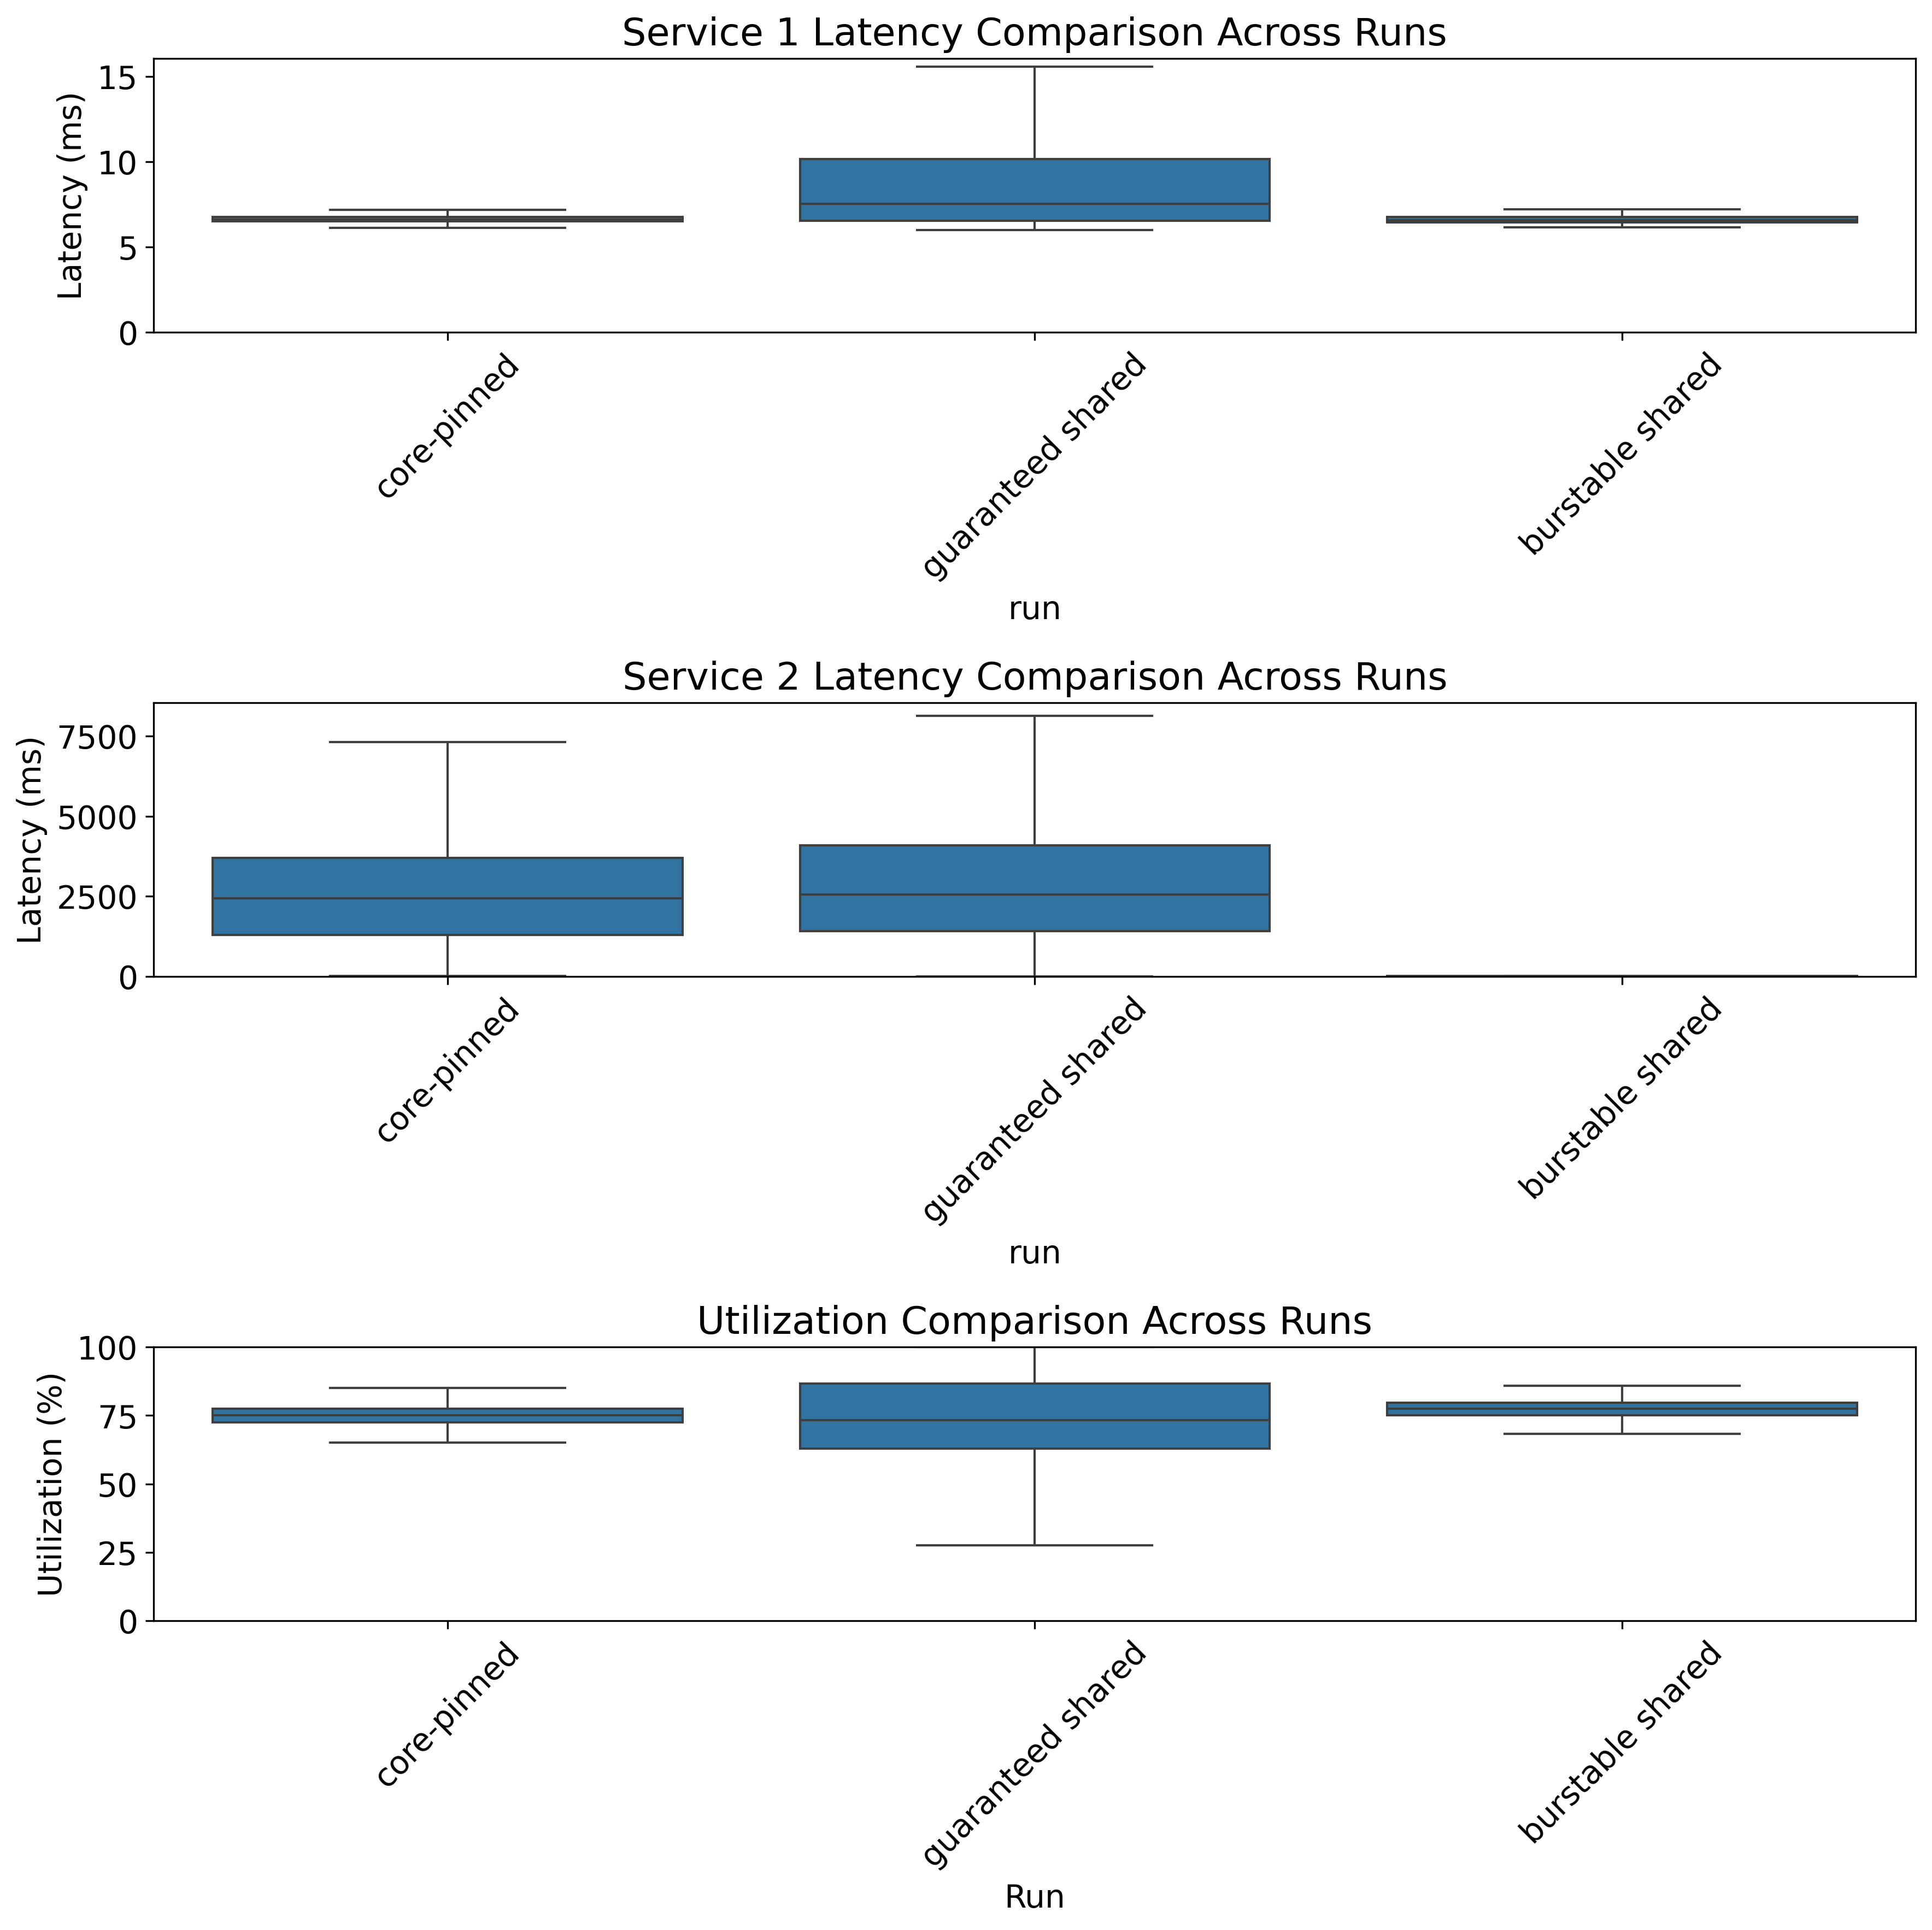
\includegraphics[width=\columnwidth]{graphs/kubernetes-lc-lc-cmp.png}
    \caption{In Kubernetes, running anything alongside a server in the
    Guaranteed QOS class affects the server's
    performance}\label{fig:kubernetes-qos-cmp}
\end{figure}

However, we find that current popular scheduling systems fail to properly
enforce reservations. We use as a case study a small but realistic social
network web application, which we run using Kubernetes.
\autoref{fig:kubernetes-qos-cmp} shows that running anything, even another
guaranteed service, alongside the web server affected its end-to-end latencies,
and that these effects go away when using core-pinning.\hmng{edited up to here}

Understanding why Kubernetes fails to honor the web application's reservation
requires looking at the underlying mechanism enforcing the CPU reservation:
Linux's \cgroups{}. In fact, most modern containers rely on \cgroups{} for CPU
isolation: all Open Container Initiative (OCI) compliant containers, including
Kubernetes but also Docker, CRI-O, and containerd
do~\cite{oci-cgroups,docker-docs-cgroups,container-isolation-article}. VM
frameworks, including Firecracker, AFaas and libvirt, also rely on \cgroups{} to
manage CPU time reservation~\cite{firecracker-cgroups,afaas,libvirt-cgroups}.

Weight is the part of the \cgroups{} interface these systems use for enforcing
the reservations LC applications have, while still allowing BEs without
reservations to run opportunistically.\footnote{Other operating systems expose a
similar interface, for instance Windows exposes a number of shares.} Kubernetes
creates one top level group for all best effort services, called
\texttt{kubepods-besteffort}, inside which all BE pods are placed, and assigns
it the lowest possible weight of 1. Pods with reservations are separated into
Burstable and Guaranteed, the main difference being that Guaranteed pods require
a limit to be set on the resources it can use. Kubernetes calculates the weight
that each pod gets based on the amount of milliCPUs it requests. For instance,
in the \autoref{fig:kubernetes-unedited} experiment, the web application service
ran in the Guaranteed class and asked for 4 CPUs, and Kubernetes assigned the
underlying pod a weight of 157.

The \cgroups{} documentation specifies that each group should get CPU time
proportional to its weight as a share of the sum of weights of runnable
groups~\cite{cgroups-kerneldocs}. However, the latency increase we see after
starting the best effort tasks in \autoref{fig:kubernetes-unedited} is much more
than the 1\% CPU time the server should be losing out on based on its weight. As
we show in more detail in \autoref{s:problem}, the problem that leads to the
increased latencies observed is that Linux will run a low weight process on one
core, unaware that a high weight process is runnable and waiting on another.
This happens because Linux uses per-CPU runqueues, which avoids the overheads of
having a global runqueue. A key challenge this work addresses is managing this
tension between how often the scheduler has to look at all the other cores'
runqueues to enforce reserved processes' priority globally, while still running
best effort ones opportunistically.

Our approach addresses this challenge by creating a new priority class for best
effort tasks to run in, \beclass{}, and enforcing it in the scheduler via
priority scheduling. Linux already has other classes between which it enforces
strict priority, which are designed and used for real time applications
(\autoref{ss:approach:linux-classes-isolate}); the proposed \beclass{} sits
below the default scheduling class. As we show in
\autoref{ss:approach:solves-problems}, putting best effort processes in a
separate class from those with reservations makes it viable to enforce those
reservations across cores, because it reduces the number of times the scheduler
is required to look at all the other cores' runqueues. Enforcing weights across
cores requires the scheduler to do so every scheduling tick, but with a separate
class it only has to look at other cores on \textit{class boundary crossings}:
every time a core switches from running an LC process to running a BE on, and
every time it enqueues an LC process.

A challenge with creating a separate priority class arises when the LC class is
under high load: completely starving best effort processes can lead to issues
such as deadlocks, broken TCP connections, or missed timers. The goal is to make
the priority of processes with reservations over those without as strict as
possible, while still allowing BE processes to resume execution normally once
the load goes down, even if the high load lasts for multiple minutes.

We address this challenge by enabling best effort processes to exist in an
ephemeral state called \textit{parked}, which they enter when the CPU
utilization is high enough that processes with a reservation account for all the
CPU time. While load remains high, the scheduler ensures that the parked BE's
user-space process doesn't run and consume resources, but continues to run the
kernel-space handlers that manage critical state, including TCP connections and
timers, on behalf of the BE processes. 

We implement \beclass{} in Linux on top of an existing scheduling policy called
\schedidle{}, and show that it is able to significiantly improve Linux's ability
to honor reservations while sharing CPUs with best effort workloads: in the same
Kubernetes experiment, the increase in average latency when starting a BE
workload goes from $>$2x to 0. The contributions of this paper are thus as
follows: 
\begin{enumerate}
    \item identifying as the reason LC tasks' reservations are often violated is
    that \cgroups{} does a poor job of enforcing the weights across cores;
    \item the design of \beclass{}, a new class for best effort tasks whose goal
    is to enforce reservations in the presence of BE processes by using priority
    scheduling, that reduces the points in time it needs to look at other core's
    runqueues, as well as enforcing the parked state
    \item an implementation of \beclass{} in Linux
\end{enumerate}


\section{Why}
\label{sec:why}

In order to understand why this is happening, we examine a trace of the
experiment. We use schedviz~\cite{schedviz}, a tool that visualizes perf traces,
to examine the scheduling decisions Linux is making.

\begin{figure*}[t]
    \centering
    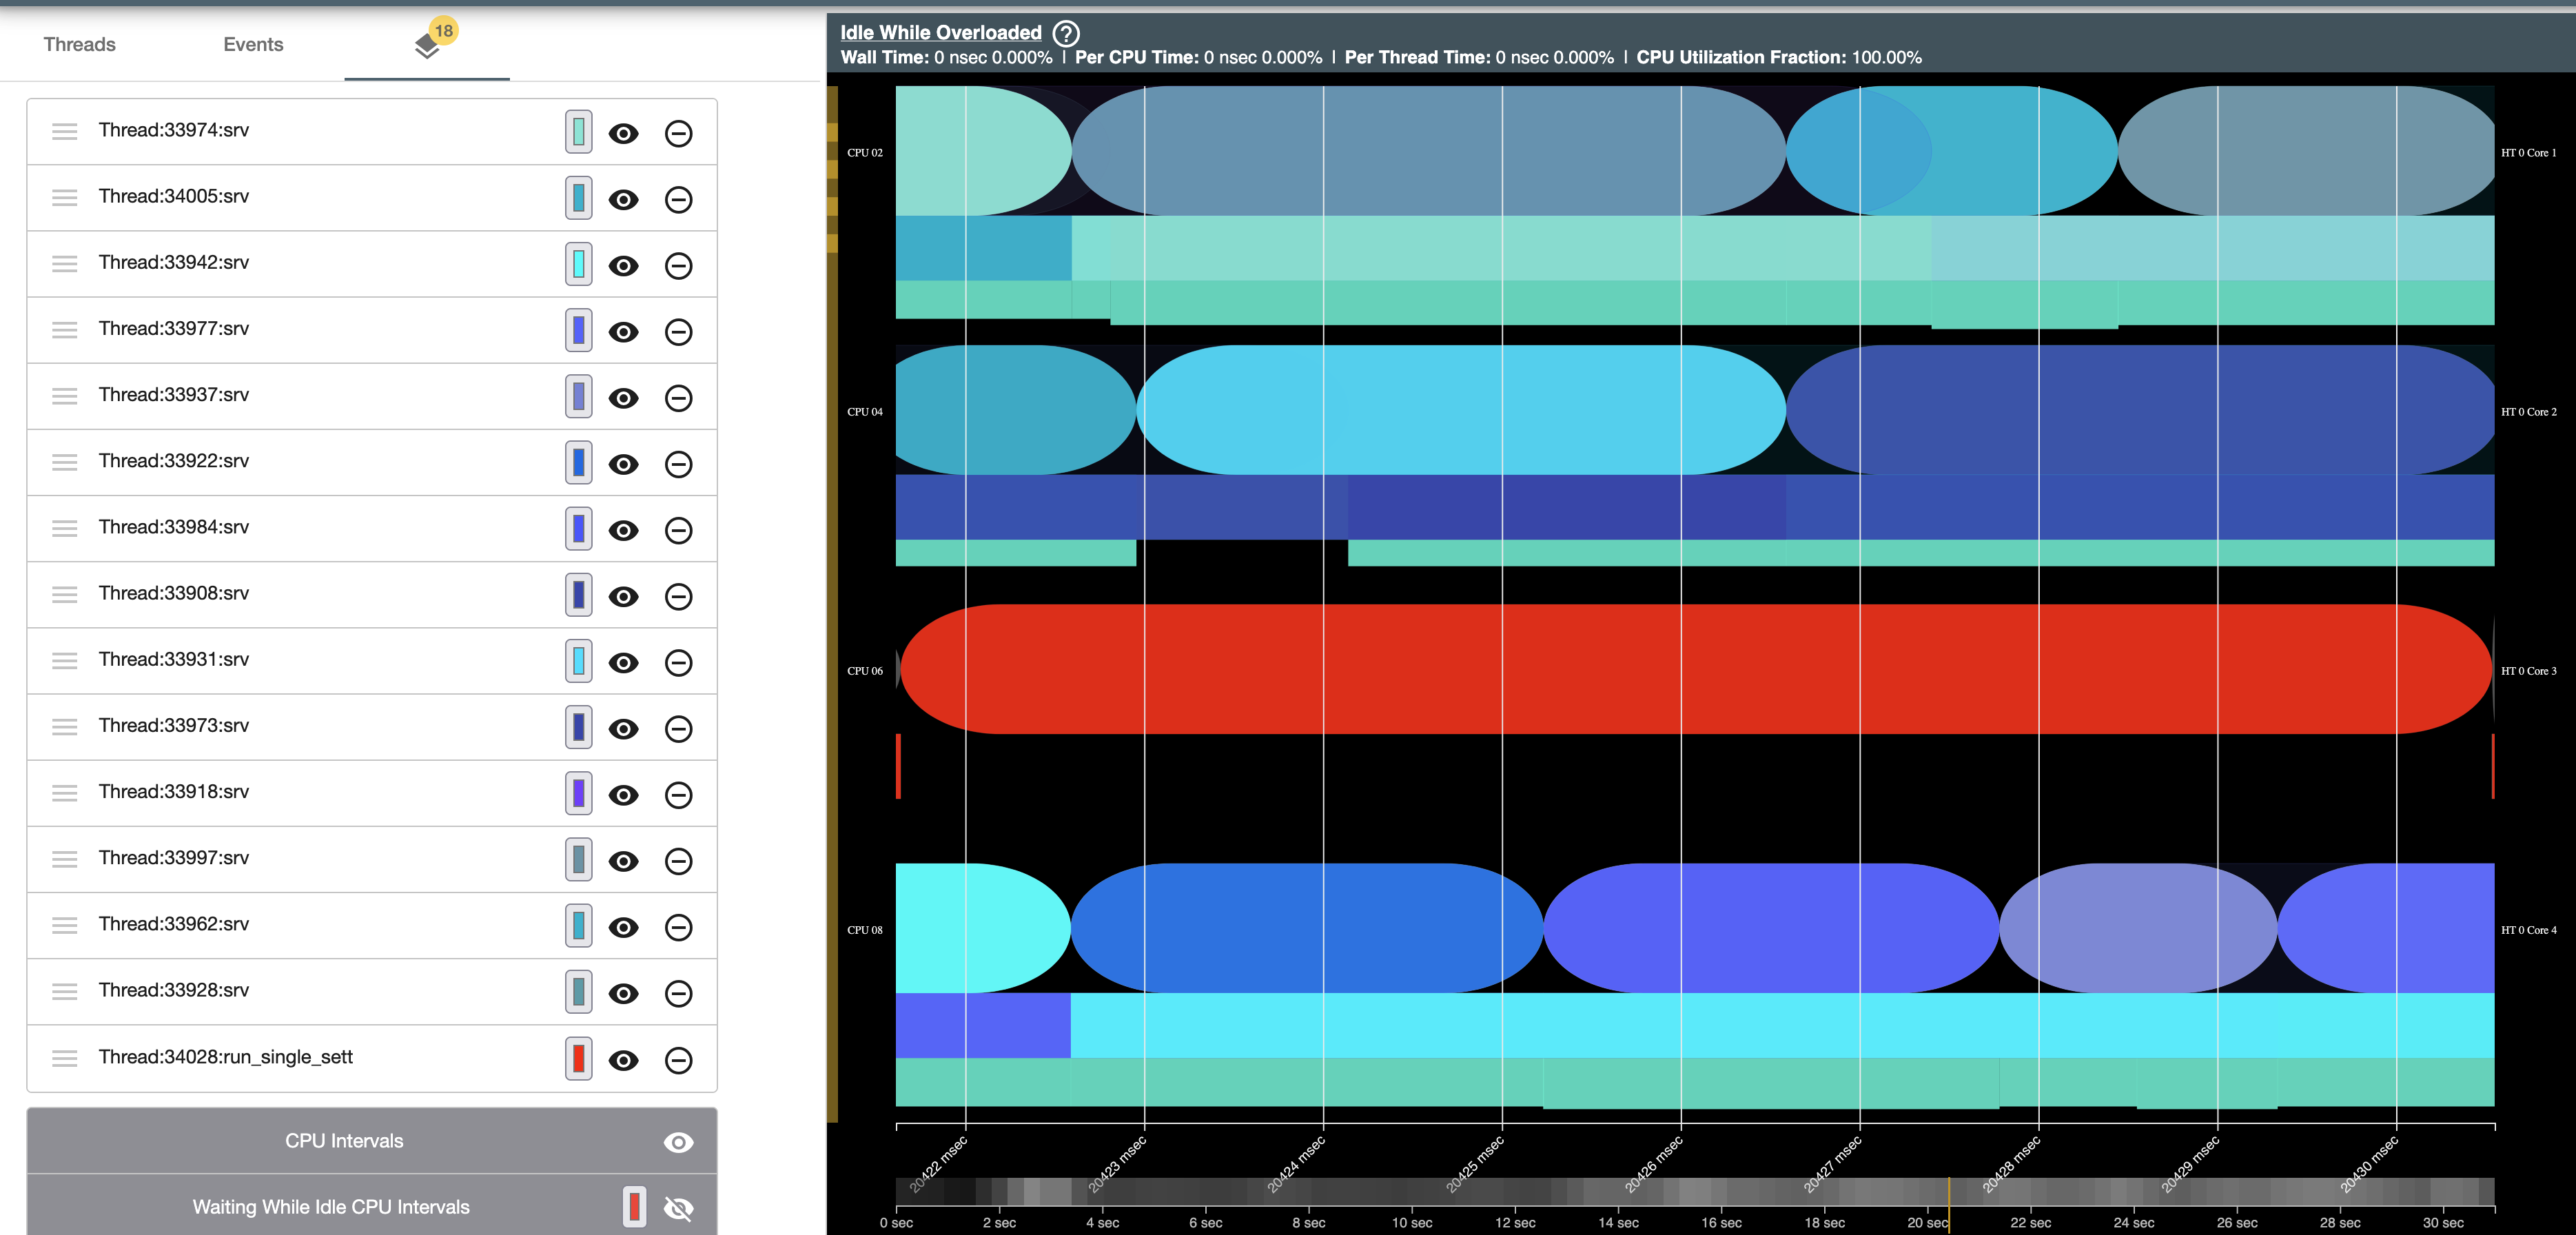
\includegraphics[width=\textwidth]{graphs/schedviz.png}
        \caption{Each thread is a different color. Circles represent which
    thread is running on that core, while rectangles underneath show waiting but
    runnable threads. Core numbers are 2,4,6,8 because this was run on a NUMA
    node so those are the cores that are closest to each other
    }\label{fig:schedviz}
\end{figure*}

In figure~\ref{fig:schedviz}, we look at a 10ms outtake from one of the runs,
that shows the problem occurring. The undesirable behavior we see here is that,
on core 6, the red process that is running the whole time is a BE process. All
the active server threads, shown in varying shades of blue, are on the other
cores, running and, more importantly, waiting.

The reason this happens is that Linux maintains a separate runqueue on each
core. This avoids the synchronization overheads of accessing global state for
every scheduling, but also means that the weight is only strictly enforced
within the individual runqueues, ie within each core. This leads to the depicted
failure mode, where an LC task is waiting on one core while another runs a BE
task.

% \hmng{should I also mention the giving at minimum 4ms? and how that can impact
%  tail latency}


\section{Real time scheduling}\label{s:realtime}

There is a way to configure tasks so that Linux enforces global priorities:
processes that run in real time have strict priority over other processes.

Linux implements real time scheduling alongside the usual weighted fair share by
supporting different \textit{scheduling classes}. There are three scheduling
classes that are accessible to users, listed in descending order of priority:
Deadline, Fifo, and Normal. Generally speaking most load is expected to fall
into the Normal scheduling class (hence the name). It is the default scheduling
class, and it is only within the Normal scheduling class that the cgroup
cpu.weight interface is relevant.

Each scheduling class exists completely separately: classes maintain their own
run queues and per-entity state; implement their own scheduling algorithms to
choose from the entities on their runqueue; and balance the load across
runqueues on different cores.

Linux isolates strictly between different scheduling classes: it only schedules
a lower scheduling class if the higher scheduling classes found nothing to run,
and each scheduling class tries to steal work from other cores before returning
that it has nothing to run. It is thereby true that if something in the Normal
scheduling class is running, it means there are no Fifo tasks waiting to run
anywhere on the machine.

This global enforcement is not succeptible to the 4ms granularity. This is
because Linux is also able to schedule at other points in time, not just the 4ms
hardware ticks. These occur when the control flow is in the kernel anyway, and
include the \textit{exit} path, when the running thread blocks, and
\textit{entry}, when a sleeping thread is woken up (via a separate signal, for
example receiving a packet on a listening socket). In these contexts Linux is
able to make fast scheduling decisions, and scheduling at these events is
sufficient to enforce isolation: the tick-based preemption granularity is
relevant for latencies of the processes within a priority, but isolating across
priorities only requires the correct scheduling decision to be made on entry and
exit. 

\begin{figure}[t]
    \centering
    \begin{subfigure}[t]{0.48\columnwidth}
        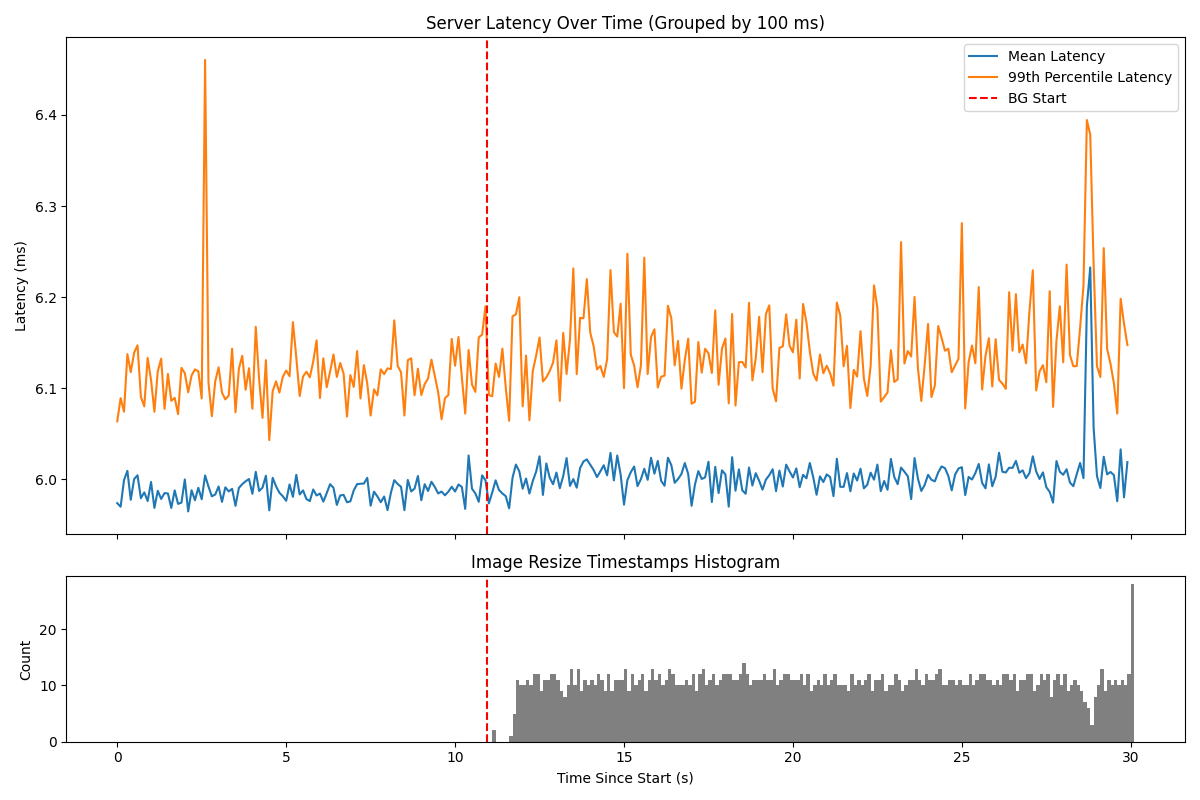
\includegraphics[width=\columnwidth]{graphs/unedited-rt-low-two.png}
        \caption{Low load}\label{fig:unedited-rt-low-two}
    \end{subfigure}
    \hspace{\fill}
    \begin{subfigure}[t]{0.48\columnwidth}
        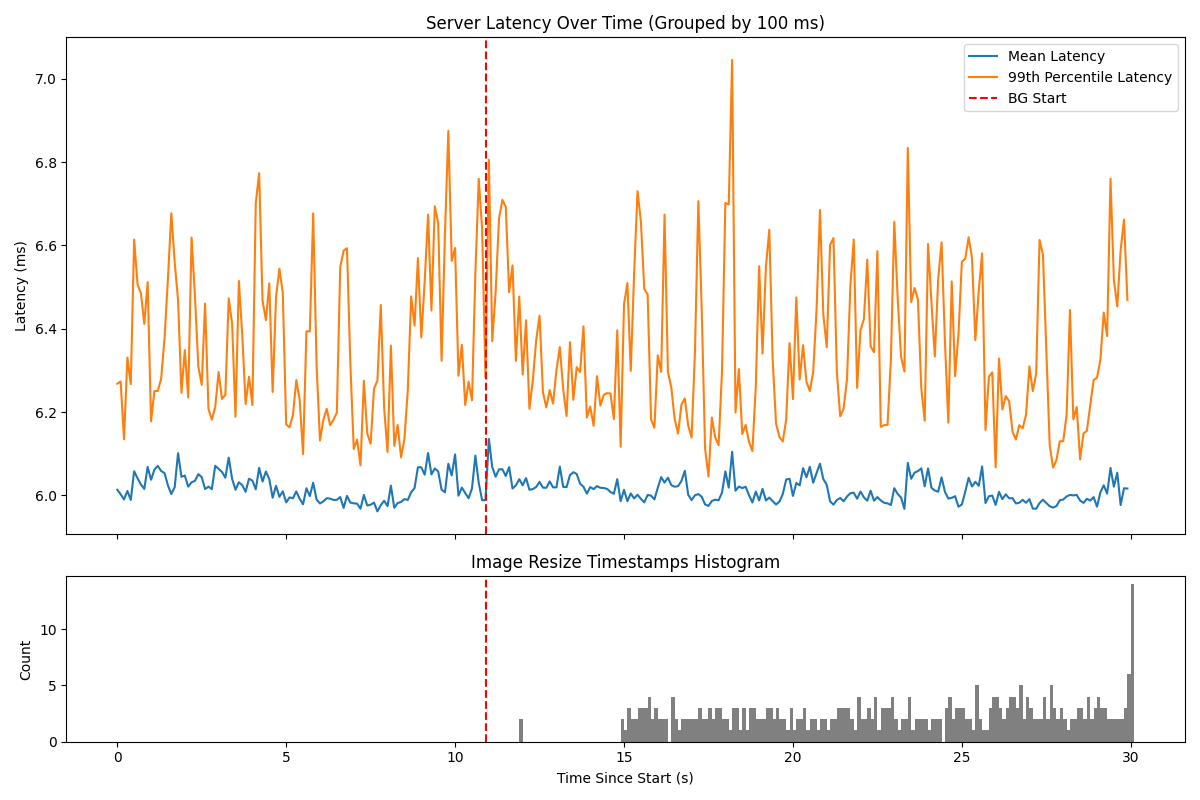
\includegraphics[width=\columnwidth]{graphs/unedited-rt-high-two.png}
        \caption{High load}\label{fig:unedited-rt-high-two}
    \end{subfigure}
    \vspace{4pt}
    \caption{Results of the same experiment, with LC running as a real time process}\label{fig:unedited-rt}
\end{figure}

This points to a possible solution: run LC in a realtime scheduling class and BE
in Normal. The Deadline class requires processes to specify a runtime $r$,
deadline $d$, and a period $p$; it guarantees that each process will get $r$
cputime by $d$, every $p$ time. So if the $r$ is 2ms, $d$ is 3, and $p$ is 10,
the Deadline scheduler guarantees that the process will get 2 ms every 10ms,
within 3ms of the period starting. The Deadline scheduler does admission control
in order to be able to make these guarantees. The Fifo scheduling class, on the
other hand, allows for oversubscription. It is a priority scheduler: it has 99
priorities, each takes strict precedent over the one lower; within priorities
the scheduler enforces a global first-in-first-out (hence the Fifo class name),
based on when processes become runnable.

So, we run the same experiment as in \autoref{s:intro}, but put the
LC task in the Fifo scheduling class, and don't put the BE tasks into groups.
Doing so effectively promotes the latency criticality of the LC task in the eyes
of the system, and makes use of Linux's strong isolation of real time workloads.
\autoref{fig:unedited-rt} shows the resulting measured latencies in the same
low and high load setting as previously. We see much stabler latencies, as
expected; in the baseline as well as once the BE tasks are started. This looks
promising on two fronts: 1: we get better isolation by making use of Linux's
strict boundaries between scheduling classes, and 2: we see improved tail
latency for the LC task because of the fifo run-to-completion scheduling
algorithm.

\begin{figure}[t]
    \centering
    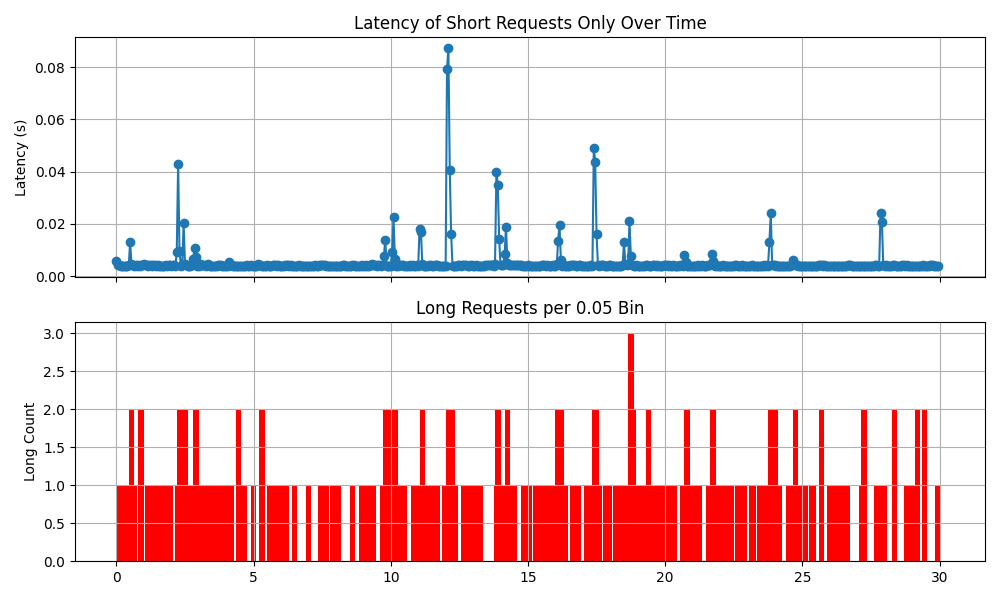
\includegraphics[width=\columnwidth]{graphs/hol-blocking.png}
    \caption{Blah blah blah}\label{fig:hol-blocking}
\end{figure}


However, the observed improved tail latency is actually a side-effect of the
experimental setup, where each request does the exact same thing and processing
times are uniform. Fifo's run-to-completion scheduling is known to have a
failure mode of head-of-line (HoL) blocking, where long-running requests
monopolize the CPU while short requests wait in the queue. This leads to much
worse tail latencies for short requests, at the expense of long requests being
slightly faster (proprtionally a smaller amount than the short requests are
waiting). We can see this phenomenon in a separate experiment, where we make a
small percentage (2\%) of requests take longer, and then graph the latencies of
only the short requests. Figure~\ref{fig:hol-blocking} shows the results, we can
see exactly when there are enough long requests that all the cores are blocked
processing them and the short requests' latencies spike. In real applications
requests almost always have a distribution of runtimes, sometimes long-tailed
sometimes short-tailed, but definitely enough of a tail that head-of-line
blocking would become a problem.

Solving the problem of HoL blocking is possible but requires knowing about
expected processing times and ensuring that requests on the same core have about
the same processing time. There is related work that does this~\cite{TODO}; but
requires a whole distributed infrastructure. The solution approach of using the
Fifo scheduler would thus require a whole infrastructure above it to minimize
the variance of processing times on cores/machines; given the original problem
was separating the LC and BE worklaods on a machine, this moves beyond the scope
of the problem.

The solution is also overkill in another dimension: Fifo enforces not only
cross-core isolation between different priorities, but also within the same
priority. This means that Linux is performing balancing and potentially
migration almost every time an LC thread wakes up or exits; in order to ensure
that the next process the core runs is next in the global fifo ordering. This
requires the scheduling core to potentially lock the runqueues of all the other
cores as it ensures the task it will run the next is the one with the highest
priority, and within that priority the once that first became runnable.\hmng{the
uptick was visible in the last graph, I think because of the spikes now it's
not. Should I try stuff to see if I can get that back?}

We conclude that the Fifo scheduling class is not a good solution: although it
is able to globally ensure isolation between LC and BE tasks, its scheduling
time overheads and algorithm make in poorly suited for a production setting.





\section{\schedidle{}: Half a scheduling class}\label{s:idle}

It now clear that what we want is the same global isolation between scheduling
classes that the using Fifo gives, but without the side-effects of the Fifo
scheduler itself. We are thus faced with an alternative of, rather than moving
the LC workload up a class, moving the BE workload down.\hmng{I kind of hate
this}

This takes us to \schedidle{}, which is the scheduling \textit{policy} that was
mentioned in \autoref{ss:intro-cgroups}. Policies are not full scheduling classes, but
allow for special casing within a scheduling class. The Normal scheduling class
supports two policies: \schednormal{}, the default, and \schedidle{}. Because
both policies are in the same class the scheduler for the Normal class is in
charge of both: it keeps the tasks of both policies on the same runqueue, and
they are all scheduled using the same algorithm. Thus, \schedidle{} is in
principle not very different from just being a low-weight process: From the
scheduler's perspective, \schedidle{} entities are just entities with a
predefined low weight (currently 3).

There is, confusingly, also an Idle scheduling \textit{class}, but that not
accessible to userspace and exists solely to manage the core's transition in and
out of being actually idle (ie running nothing).

The main way that the Normal scheduler special-cases \schedidle{} entities from
\schednormal{} entities is during wakeup: in a 2019 patch~\cite{TODO}, Linux
added a check where, when a \schednormal{} entity becomes newly runnable, if the
core where the entity is waking up is already running something in
\schednormal{}, it will look for other cores that might be currently running a
\schedidle{} entity, and migrates the new entity there.

In doing so, Linux created a half scheduling class. As discussed in
\autoref{s:realtime}, in order to fully isolate two groups of processes the
scheduler needs to try synchronize across cores at two points: entry and exit.
The described patch adds only the entry check.

\schedidle{} is additionally promising because, as we saw in
\autoref{ss:intro-cgroups}, it was extended to have cgroup support
recently\cite{TODO}: when set via the cpu.idle cgroup interface file, the entire
cgroup is counted as a \schedidle{} entity. This means that rather than needing
to set the scheduling policy from within each process, a solution that uses
\schedidle{} would be able to rely on the usual mechanism of using the
\cgroups{} interface.

\begin{figure}[t]
    \centering
    \begin{subfigure}[t]{0.49\columnwidth}
        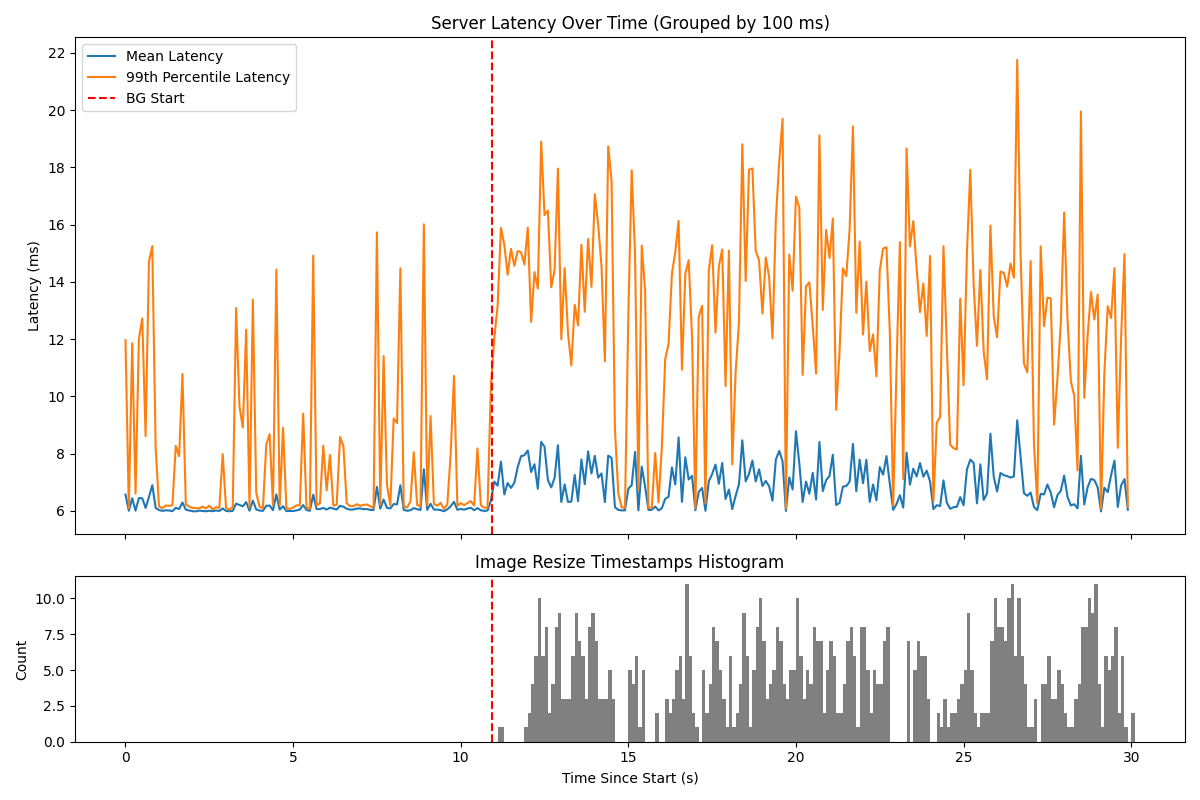
\includegraphics[width=\columnwidth]{graphs/unedited-idle-low-two.png}
        \caption{Low load}\label{fig:unedited-idle-low-two}
    \end{subfigure}
    \hspace{\fill}
    \begin{subfigure}[t]{0.49\columnwidth}
        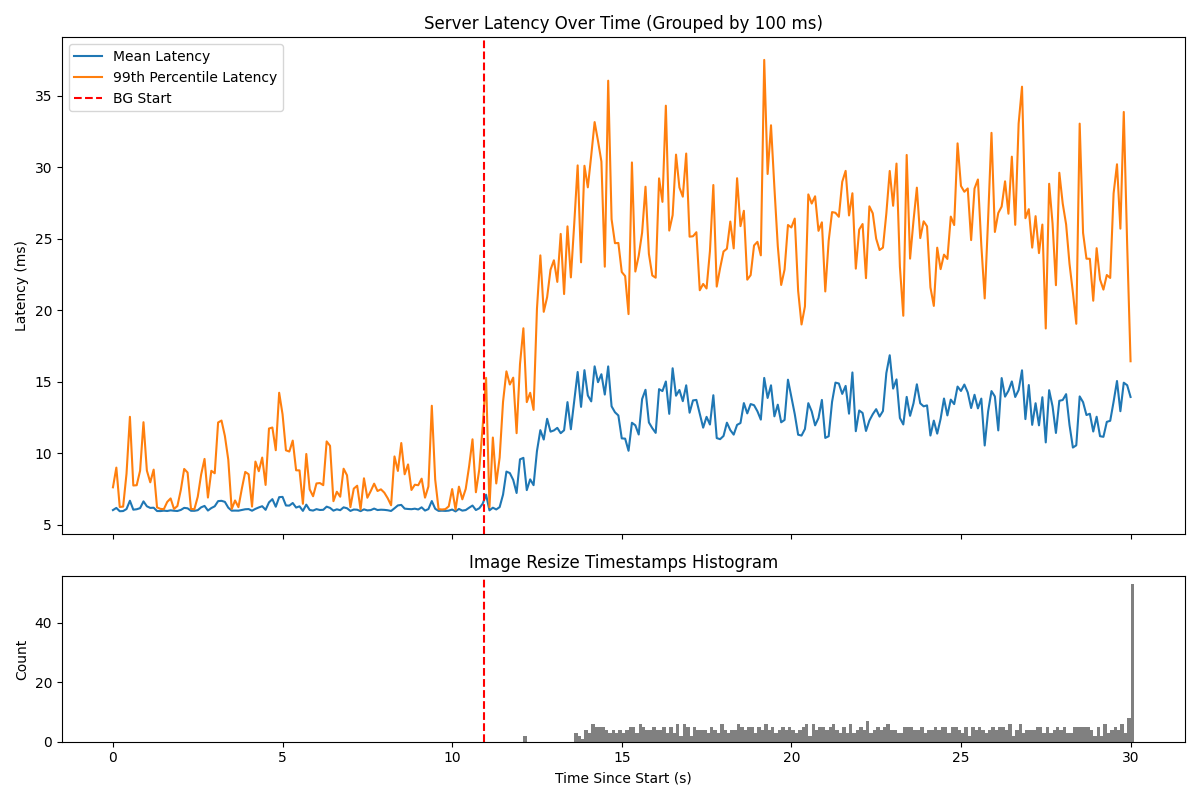
\includegraphics[width=\columnwidth]{graphs/unedited-idle-high-two.png}
        \caption{High load}\label{fig:unedited-idle-high-two}
    \end{subfigure}
    \vspace{4pt}
    \caption{using \schedidle{}}\label{fig:unedited-idle}
\end{figure}

And indeed, we find that when we use cgroups' new cpu.idle interface feature,
the latency impact of the BE tasks decreases, although it does not entirely drop
to what we saw with the Fifo class.\ \autoref{fig:unedited-idle} shows the
results, for the familiar settings of low and high load. The jump we see in the
mean latency has decreased from peaks as high as 13ms to around 7ms (even though
in principle they now have a higher weight).



\section{Using \priceclass{}es in \Sys}\label{design}

This section describes \sys{}, a scheduler that addresses the \problem{} using
\priceclass{}es, and addresses the \autoref{s:intro} challenges.

\subsection{\Priceclass{}es}

\Sys{} uses \class{}es to supplant the current interface, which requires
developers to choose an amount of memory per function (which is then tied to a
CPU fraction, \eg{} 0.2 vCPUs).  \Sys{} bills memory separately and by use, and
the price for memory is the same across all \class{}es.

\Priceclass{}es don't imply absolute guarantees about what resources a function
receives.  The \priceclass{} is instead a metric to express priority to \sys{},
which \sys{} uses to enforce a favoring of high \class{} functions.  To avoid
the developer-side uncertainty of bidding wars, \sys{} exposes a fixed set of
\priceclass{}es (similar to how AWS has different EC2 instance types).

\Priceclass{}es are a metric that has a number of benefits over resource usage
estimations. One is that developers are more likely to have a good sense of what
\priceclass{} a function should have ahead of time, because they know in what
context the function will be used. \Priceclass{}es also remain the same across
different invocations, whereas resource needs can be heavily skewed in web
applications~\cite{hermod,serverless-in-the-wild}. And finally, \class{}es more
directly align the interests of the developer with those of the provider, by
communicating on the level of what the provider and developer actually care
about: money, and latency (as achieved by \class{}es in the system).

\Priceclass{}es also allow the provider to provision their datacenters hardware:
by looking at the historical overall amount of high \priceclass{} load, they
know a minimum of how much hardware they need to buy to be able to comfortably
fit that load.

\subsection{Interface}

Developers using \sys{} write function handlers and define triggers just like
they would for existing serverless offerings.  Triggers assign a \priceclass{}
to a function invocation based on the function and its arguments.
For instance, a simple web application might consist of a home page view that is
assigned a higher \priceclass{} and costs 2$\mu\cent$ per cpu second, a user
profile page view which is assigned a middle-high \class{} and costs
1.5$\mu\cent$ per cpu second, and finally an image processing function that can
be set to a low \class{} which costs only 0.5$\mu\cent$ per cpu second.

\Class{}es are inherited across call chains: if a high \class{} function calls a
low \class{} function, that invocation will run with a high \class{}. This
inheritance is important in order to avoid priority inversion.

To avoid unexpected costs in the case of, for example, a DOS attack or a bug,
developers also express a monthly budget that they are willing to pay.~\Sys{}
uses this budget as a guideline and throttles invocations or decreases quality
of service in the case that usage is not within reason given the expected
budget, though it does not guarantee that the budget will not be exceeded by
small amounts.

\subsection{\Sys{} Design}

\begin{figure}[t]
    \centering
      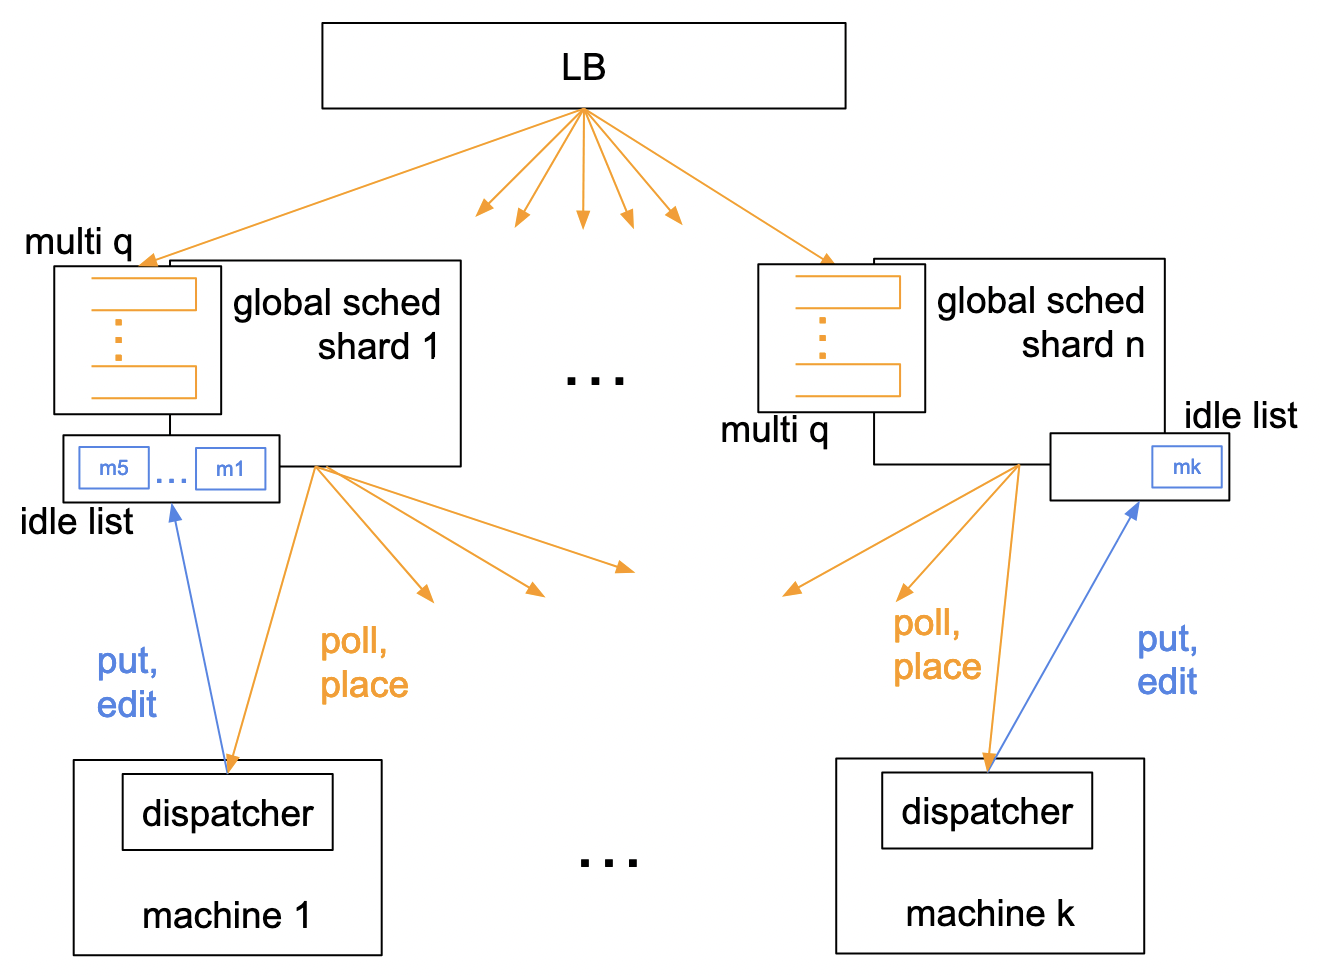
\includegraphics[width=8.5cm]{img/overview.png}
      \caption{ global scheduler shards queue and place functions (in orange),
      on each machine a dispatcher thread keeps track of memory utilization and
      writes itself to idle lists (in blue) }
    \label{fig:overview}
\end{figure}



\Sys{} has as its goal to enforce the \class{}es attached to
functions, which means it needs to prefer higher \class{} functions
over lower ones, and preempt the latter when necessary. As shown in
Figure~\ref{fig:overview}, \sys{} sits behind a load balancer, and
consists of: a \textit{distributed global scheduler}, which places new
function invocations and has attached an \textit{idle list}, a
\textit{dispatcher}, which runs on each machine and communicates with
the global scheduler shards, and a \textit{machine scheduler}, which
enforces \class{}es on the machines.


\textbf{Machine Scheduler.}
The machine scheduler is a preemptive priority scheduler: it preempts lower
\class{} functions to run higher \class{} ones. Being unfair and starving low
\class{} functions is desirable in \sys{}, since image processing functions
should not interrupt a page view request processing, but vice versa is expected.
Within \class{}es the machine scheduler is first come first served. This design
matches Linux' ``SCHED FIFO'' policy~\cite{linux-sched}.


\textbf{Idle list.}  Each global scheduler shard has an idle list,
which holds machines that have a significant amount of memory
available. In the shards idle list, each machine's entry is associated
with the amount of memory available as well as the current amount of
functions on the machine. The idle list exists because datacenters are
large: polling a small number of machines cannot find something that
is a rare occurrence~\cite{join-idle-queue}. The idle list allows the
rare idle machine to make itself visible to the global scheduler. The
idle list also allows the global scheduler to place high \class{}
functions quickly, without incurring the latency overheads of doing
polling to find available resources. This design is inspired by Join
Idle Queue~\cite{join-idle-queue}, but defines idleness via memory
availability rather than empty queues.


\textbf{Dispatcher.}
The dispatcher is in charge of adding itself to a shard's idle list when memory
utilization is low. The dispatcher chooses which list to add itself to using
power-of-$k$-choices: it looks at $k$ shards' idle lists and chooses the one with
the least other machines in it. If the machine is already on shard $i$'s idle
list, but the amount of available memory has changed significantly (either by
functions finishing and memory being freed or by memory utilization increasing
because of new functions or memory antagonists), the dispatcher will update
shard $i$'s idle list.

The dispatcher is also in charge of managing the machine's memory. When memory
pressure occurs, the dispatcher uses \textit{\class{}-based swapping} to move
low \class{} functions off the machine's memory. Having prices classes
creates an opportunity: because the dispatcher knows that the lowest \class{}
functions will not be run until the high \class{} functions have all finished,
it can swap its memory out knowing it will not be needed soon. The dispatcher
swaps the low \class{} function back in when the memory pressure is gone and the
function will be run.

\Sys{} cannot bound the amount of swap space required since it doesn't ask
functions for a memory bound.  In the rare case that memory still runs out,
\sys{} resorts to killing low \class{} functions.  Providers can estimate the
amount of swap space required by looking at memory utilization, and since the
SSDs necessary for swap space are inexpensive~\cite{ssd-price} we expect that
killing is rare.

\textbf{Global Scheduler Shards.}
Global scheduler shards store the functions waiting to be placed in a multi
queue, with one queue per \priceclass{}. Shards choose what function to place
next by looking at each function at the head of each queue, and comparing the
ratio of \class{} to amount of time spent in the queue. This policy ensures
that high \class{} functions don't have to wait as long as low \class{}
functions to be chosen next, but low \class{} functions will get placed if they
have waited for a while.

When placing the chosen function, the shard will first look in its
idle list. If the list is not empty, it will choose the machine with
the smallest queue length.  If there are no machines in the idle list,
the shard switches to power-of-$k$-choices: it polls $k$ machines, and
chooses the least loaded machine (by number of functions running).

%-------------------------------------------------------------------------------
\section{Evaluation}
\label{s:eval}
%-------------------------------------------------------------------------------

This section answers the following questions:
\begin{enumerate}
    \item Does \schedbe{} isolate LC from BE workloads?
    \item Can parked processes resume correctly? How many resources does it used
    while parked?
    \item How much does \schedbe{} cost?
    \item How does \schedbe{}'s isolation compare to that of \schedidle{}?
\end{enumerate}

All the graphs in this paper run on Linux version 6.14.2, the baseline version
that our implementation builds on.

\subsection{Does \schedbe{} isolate?}

\begin{figure}[t]
    \centering
    \begin{subfigure}{\columnwidth}
        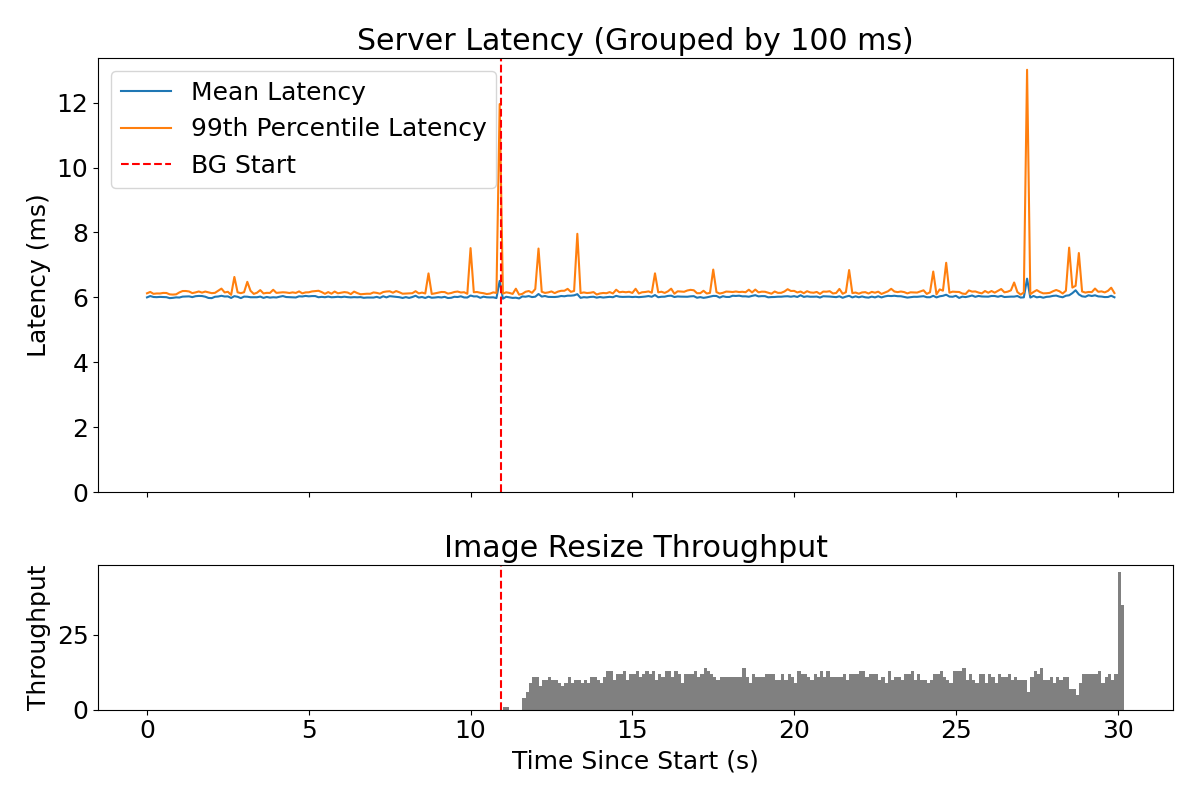
\includegraphics[width=\columnwidth]{graphs/srv-bg-schedbe-low.png}
        \caption{Low load (85\%)}\label{fig:srv-bg-schedbe-low}
        \vspace{12pt}
    \end{subfigure}
    \begin{subfigure}{\columnwidth}
        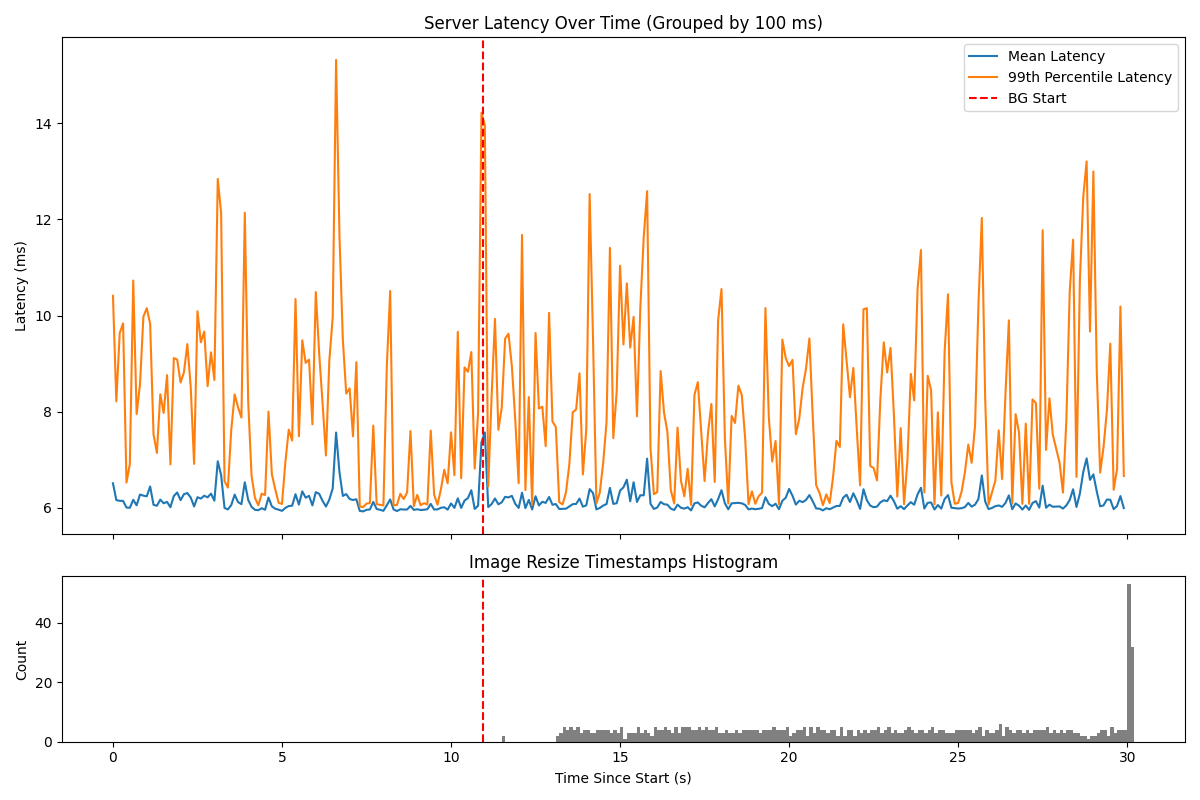
\includegraphics[width=\columnwidth]{graphs/srv-bg-schedbe-high.png}
        \caption{High load (95\%)}\label{fig:srv-bg-schedbe-high}
    \end{subfigure}
    \vspace{4pt}
    \caption{same expiriment as in \autoref{fig:srv-bg-weight-150}, but with the
    BEs running in \schedbe{}}\label{fig:srv-bg-schedbe}
\end{figure}

\begin{figure}[t]
    \centering
    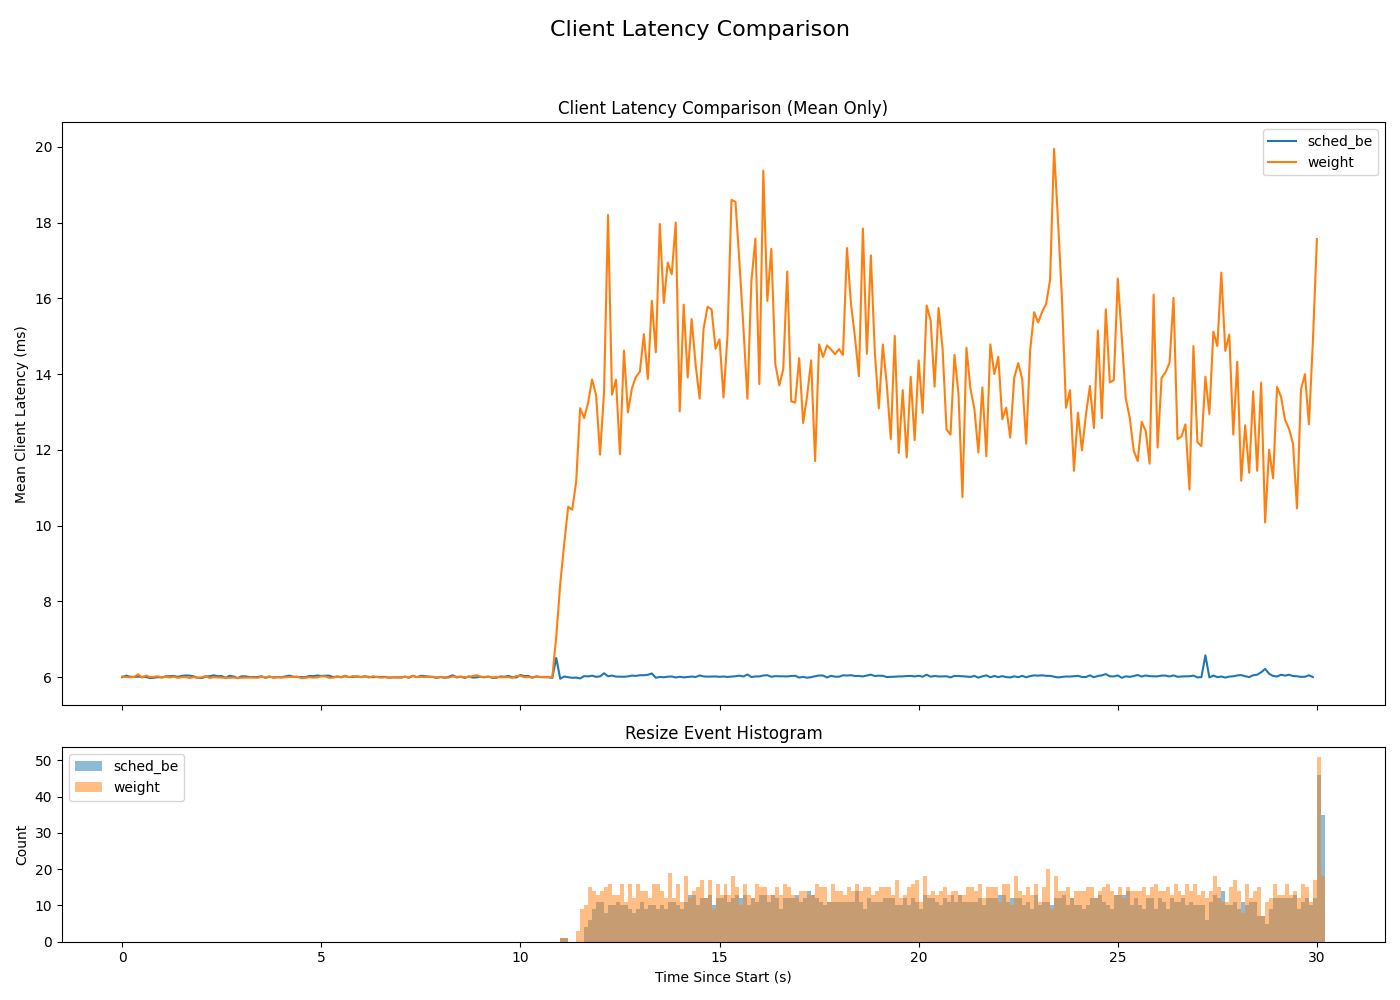
\includegraphics[width=\columnwidth]{graphs/srv-bg-cmp-unedited-schedbe.png}
    \caption{A direct comparison between the server latencies when using the
    existing \cgroups{} weights versus \schedbe{} to isolate the LC from the
    BE}\label{fig:srv-bg-cmp-unedited-schedbe}
\end{figure}

\begin{figure}[t]
    \centering
    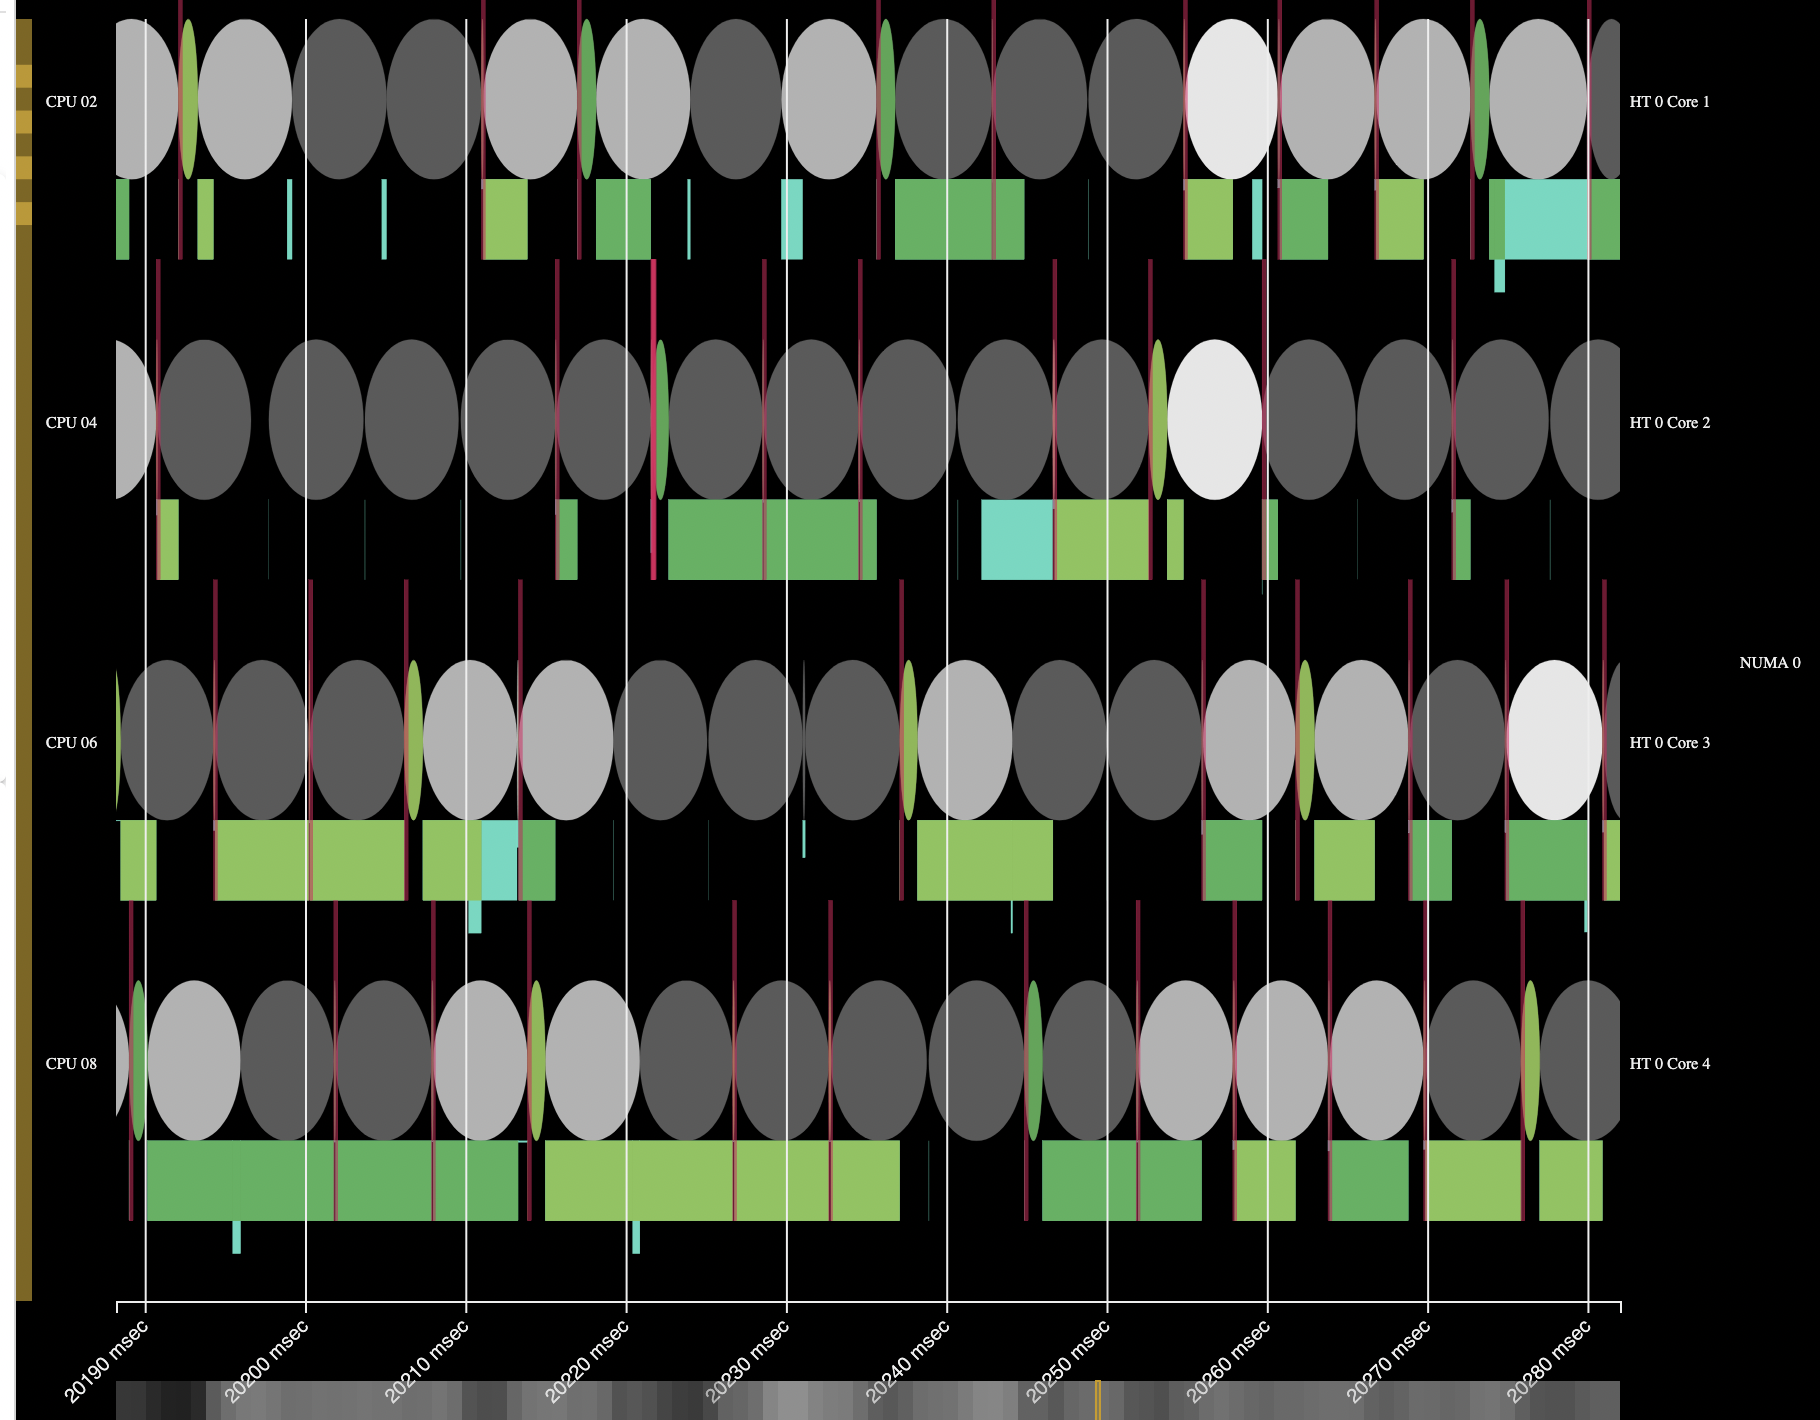
\includegraphics[width=\columnwidth]{graphs/schedviz-schedbe.png}
    \caption{BE threads only run in the gaps when there are no queued LC
    threads. The BE threads are colored in two different shades of green, the LC
    threads are the grey ones (all the threads are the same shade of grey, the
    different shades have to do with the amount of processes the visualizer has
    grouped). The red vertical lines are the scheduler initially choosing a BE
    thread, which leads to an attempt to steal a queued LC one.
    }\label{fig:schedviz-schedbe}
\end{figure}

We run the microbenchmark experiment from \autoref{fig:srv-bg-weight-150} using
\schedbe{}. We can see the resulting performance in
\autoref{fig:srv-bg-schedbe}, and \autoref{fig:srv-bg-cmp-unedited-schedbe}
shows a direct comparison between the original benchmark run on \cgroups{}
weights and running it using \schedbe{}. As desired, the latency of the server
remains stable after the background tasks start. This does not mean that the
background task never runs: the lower part of each graph still shows iterations
of image resizing being done. The difference is that now the background tasks
will reliably get interrupted when the LC server has a request to process.
\autoref{fig:schedviz-schedbe} shows this happening in an outtake of a schedviz
visualization. The green BE processes run only in the gaps where there is no
queued LC process, and are immediately preempted when one wakes up, on whatever
core that may be. The vertical red lines show when the \exit{} path \schedbe{}
introduced runs, \ie{} when the core has chosen intially to run a BE process
after having previously run LC. As we can see, this is sometimes followed by
just running the BE, but often by the core running an LC process, meaning that
it succesfully found and stole a queued and waiting LC thread.

\begin{figure}[t]
    \centering
    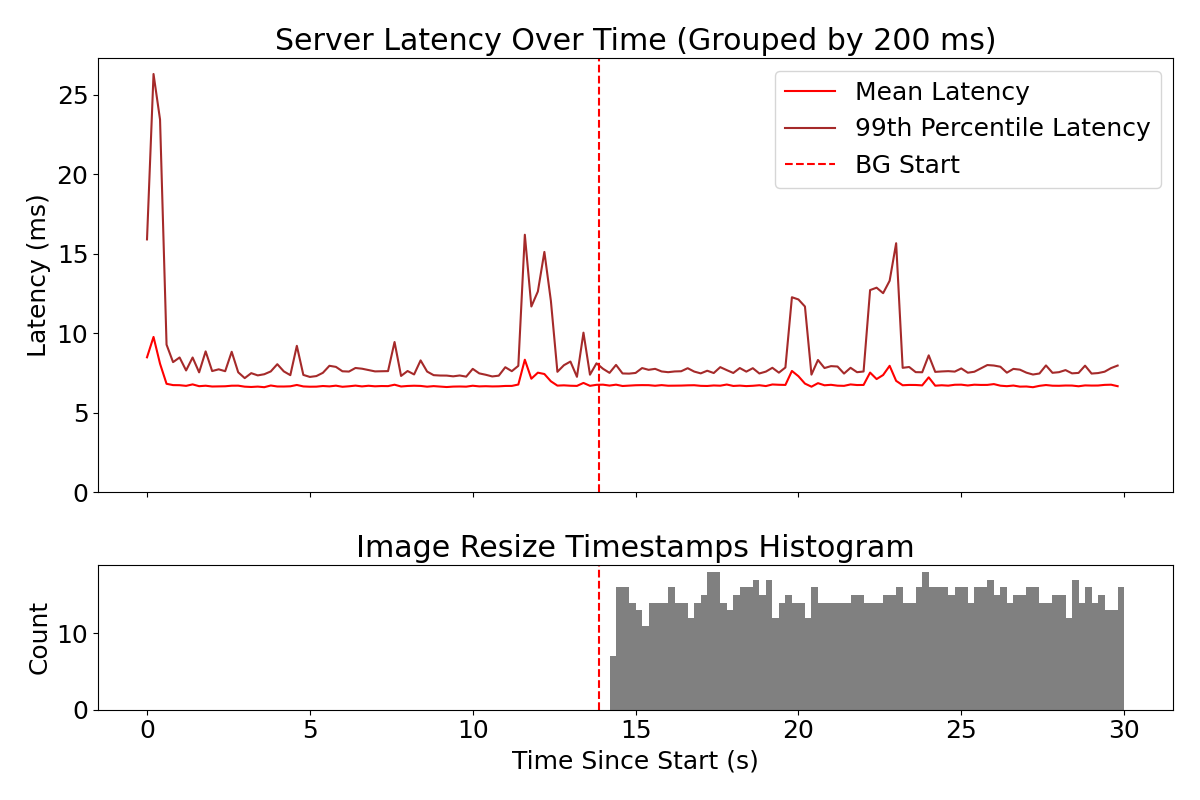
\includegraphics[width=\columnwidth]{graphs/kubernetes-schedbe.png}
    \caption{The same experiment as in \autoref{fig:kubernetes-unedited}, but
    running the BE as a \schedbe{} task}\label{fig:kubernetes-schedbe}
\end{figure}

We also run the Kubernetes application from \autoref{fig:kubernetes-unedited}
using \schedbe{}. The results are in \autoref{fig:kubernetes-schedbe}. We can
see that again the latency profile of the LC web application looks largely the
same before and after starting the image resize job.\hmng{run for longer and/or
get concrete numbers for how much it increases, vague hedging (largely, not
entirely) is not good} It is not entirely without spikes, but the spikes come
from interference with Python runtimes and Kubernetes controllers, and are the
same before and after starting the BE tasks. Importantly, the baseline median
latency of the LC web application stays stable at around 7.4ms after starting
the the BE image resizing. 

\subsection{Can parked processes resume correctly? How much do they cost while
parked?}\label{ss:eval:parking}


\begin{figure}[t]
    \centering
    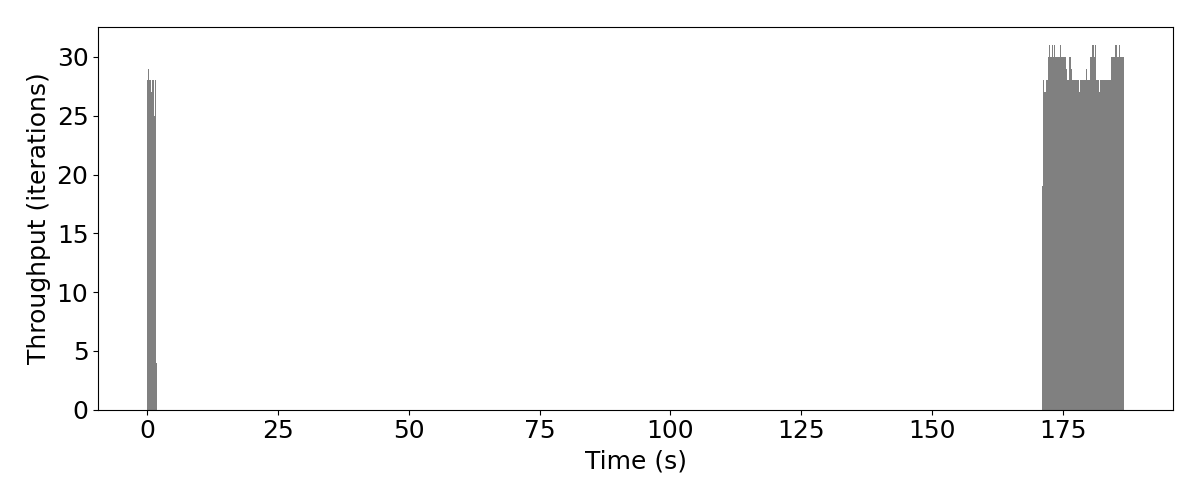
\includegraphics[width=\columnwidth]{graphs/parked-kubernetes.png}
    \caption{A \beclass{} process in a Kubernetes pod, parked while the
    antagonist runs and then resuming}\label{fig:parked-kubernetes}
\end{figure}

We investigate parking by running a BE Kubernetes pod alongside an antagonist,
and find that even after being parked for multiple minutes in the middle of
processing a request, the BE job is able to resume and return the final result
to the client. \autoref{fig:parked-kubernetes} shows the throughput over time of
an image resize job running in a BE container running as \schedbe{}. A couple
seconds after sending a request to the image resize pod, we start an entirely
CPU-bound antagonist on the same set of cores as the BE is running. We can see
that the image resize job is completely paused for about two and a half minutes,
until the antagonist is done running. The job then continues and completes. The
client connection did not experience any issues, even when setting the TCP
keepalive timeout to expire within duration the BE spent being parked.

\begin{figure}[t]
    \centering
    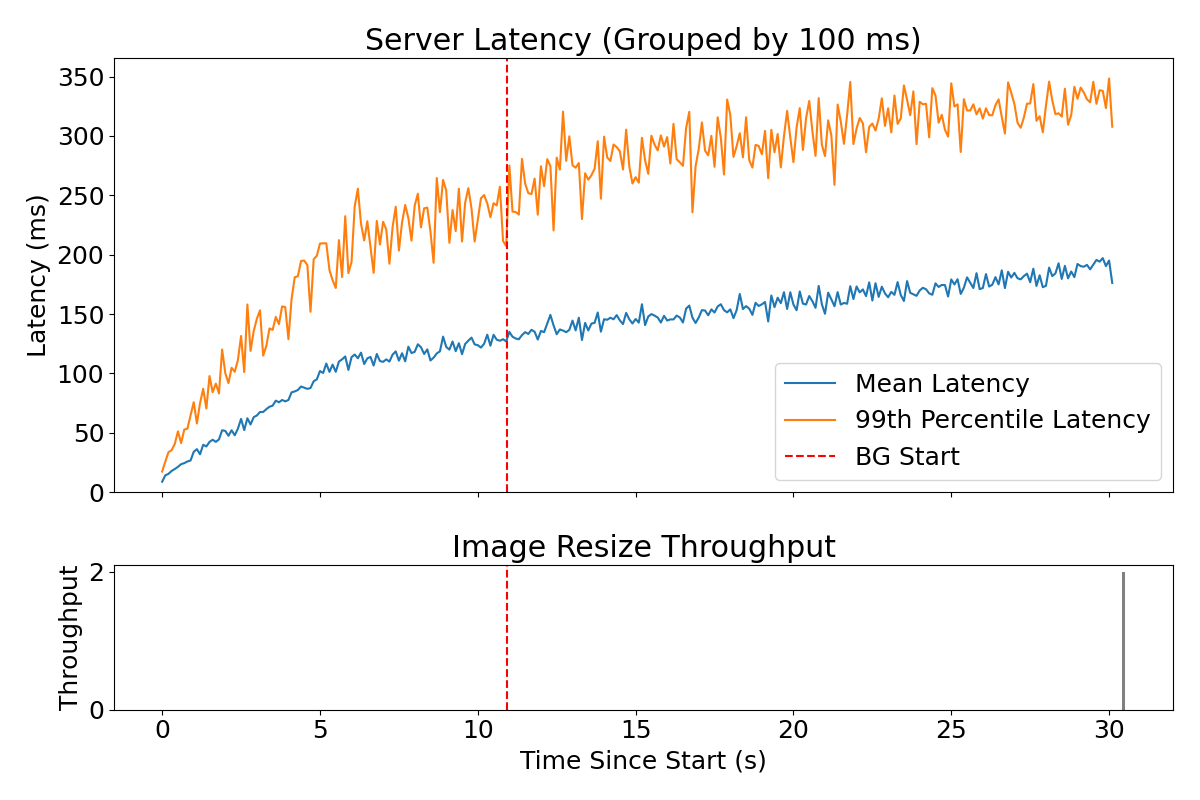
\includegraphics[width=\columnwidth]{graphs/overload-schedbe.png}
    \caption{BE in \schedbe{}, no throttling}\label{fig:overload-schedbe}
\end{figure}

\autoref{fig:overload-schedbe} shows how parking enables the LC to be isolated
from \schedbe{} even under sustained extremely high load. We run the same
experiment as \autoref{fig:overload-rt}, but now instead instead of throttling
the LC, the BE gets parked. Notice that the BE does not make progress until the
very end, when the server is done processing the requests. The difference is
stark: in both experiments, the open-loop client sent the same amount of
requests with the same amount of time in between them, but when the LC was
throttled it took the server 35s to process all the requests, with a final
latency of >1s, and with parking the server finished the client load in 31s with
a final avg latency of <200ms. 



\subsection{Cost of \schedbe{}}

The cost of \schedbe{} is can be broken down into the three checks that make up
the priority enforcement:

\begin{enumerate}
    \item \local{} adds a small amount of compute overhead on each scheduling
    decision to determine threads' priorities. This is a small amount of code we
    do not expect to impact latency
    \item \entry{} adds no new latency to Linux, which already implements
    \entry{} for \schedidle{}
    \item \exit{} adds overheads in two places: one is the cross-core check that
    each happens at each class boundary crossing, and the other is the overhead
    of the migration should it decide to steal a \schednormal{} process
\end{enumerate}

We look at how often the \exit{} check happens as well as how often it chooses
to steal in the Kubernetes experiment. The overhead of stealing the LC job is
known, and is a complicated function of the CPU architecture and which cores it
is moving between (\eg{} how much memory hierarchy do the two cores share).

% Please add the following required packages to your document preamble:
% \usepackage[normalem]{ulem}
% \useunder{\uline}{\ul}{}
\begin{table}[t]
    \centering
    \begin{tabular}{|l|l|l|}
        \hline
                & \# times runs & \# times successful \\ \hline
        \entry{} & $\sim$60K    & $\sim$12.5K         \\ \hline
        \exit{}  & $\sim$20K    & $\sim$10K          \\ \hline
    \end{tabular}
    \vspace{10pt}
    \caption{Counts of checks and how many times they run/are able to find an LC to
    run/a BE to interrupt}\label{tab:check-counts}
\end{table}

In the span of the 30 seconds the Kubernetes experiment takes to run, and across
the four cores it runs, we see the following: scheduling happens around 110K
times, which is a little less than once per ms on each core. The \entry{} check
happens $\sim$60K times, or about twice a ms. This makes sense: the client sends
a request every 2ms which will cause a server thread wakeup, and the software
stack includes Linux, Docker, and Kubernetes, all of which have worker threads.
Of those 60K \entry{} checks, 12.5K find an idle runqueue. The \exit{} check
happens fewer times, around 20K times, of which approximately half lead to
stealing a \schednormal{} task.

We can see that the \entry{} and \exit{} checks happen less than scheduling does
by more than half. This demonstrates that enforcing isolation between LC and BE
via priority classes requires much fewer cross-core checks than doing so at
every scheduling decision.

The other takeaway is that, under high load, the \exit{} check is effective:
around half of the time, the scheduler found a queued LC thread on another core.
Without the check, each of those would have led to a priority inversion.


\subsection{Comparison with \schedidle}\label{ss:eval:schedidle}

As discussed in \autoref{s:implementation}, \schedidle{} implements some but not
all of the isolation required of \beclass{}: it implements the \entry{} check,
but not the \exit{} check or strict local priorities.

\begin{figure}[t]
    \centering
    \begin{subfigure}[t]{\columnwidth}
        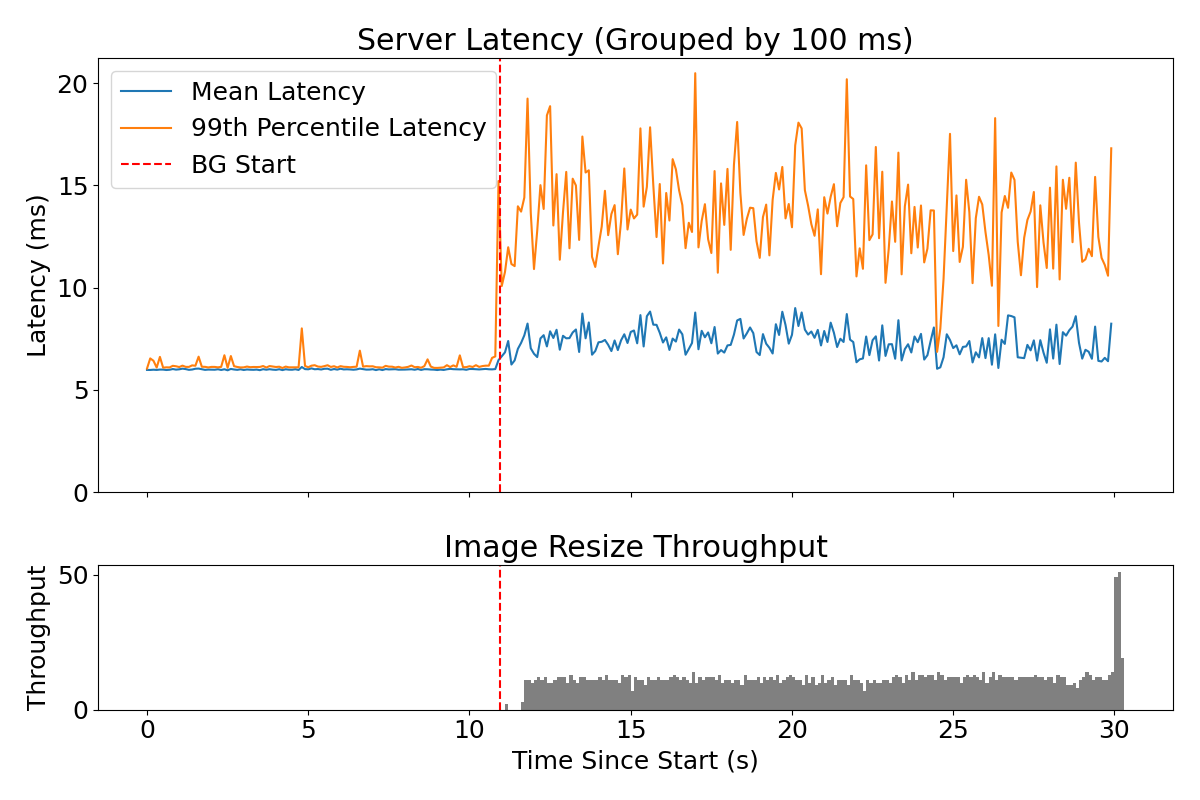
\includegraphics[width=\columnwidth]{graphs/srv-bg-idle-low.png}
        \caption{\schedidle{} in low load (85\%)}\label{fig:srv-bg-idle-low}
        \vspace{12pt}
    \end{subfigure}
    \hspace{\fill}
    \begin{subfigure}[t]{\columnwidth}
        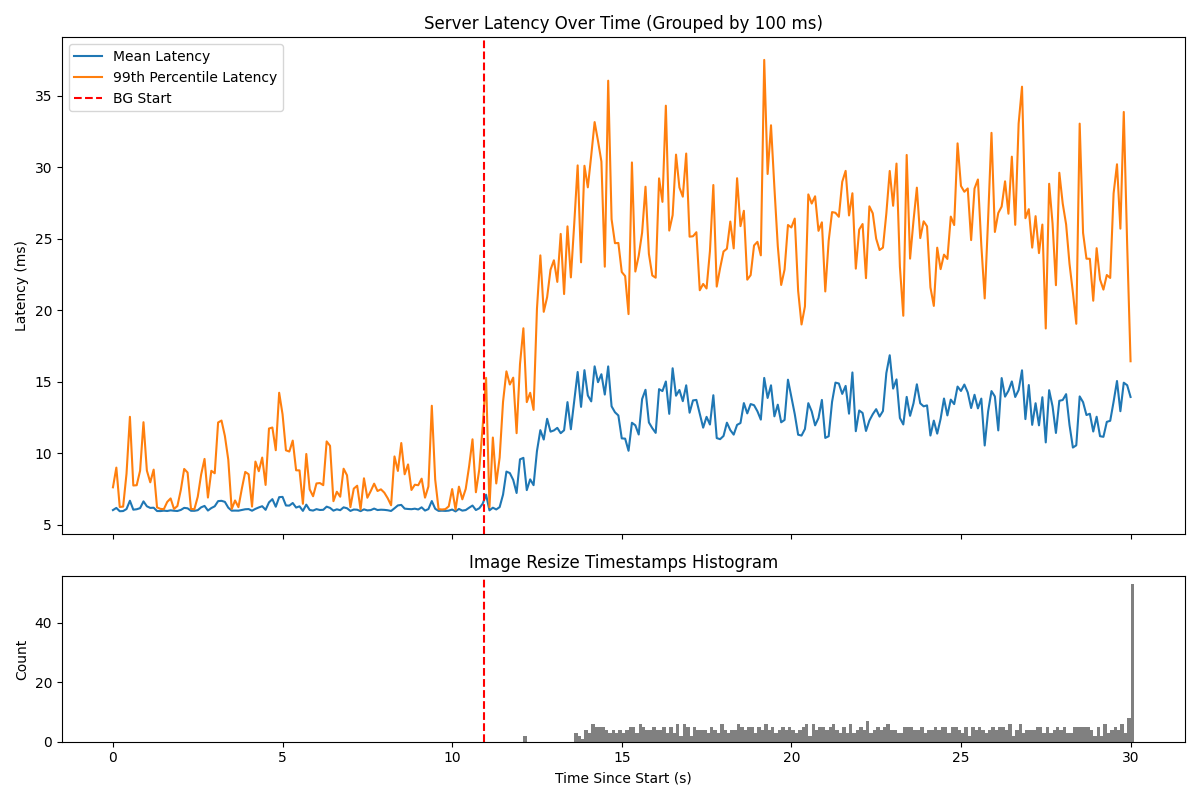
\includegraphics[width=\columnwidth]{graphs/srv-bg-idle-high.png}
        \caption{\schedidle{} in high load (95\%)}\label{fig:srv-bg-idle-high}
        \vspace{12pt}
    \end{subfigure}
    \hspace{\fill}
    \begin{subfigure}[t]{\columnwidth}
        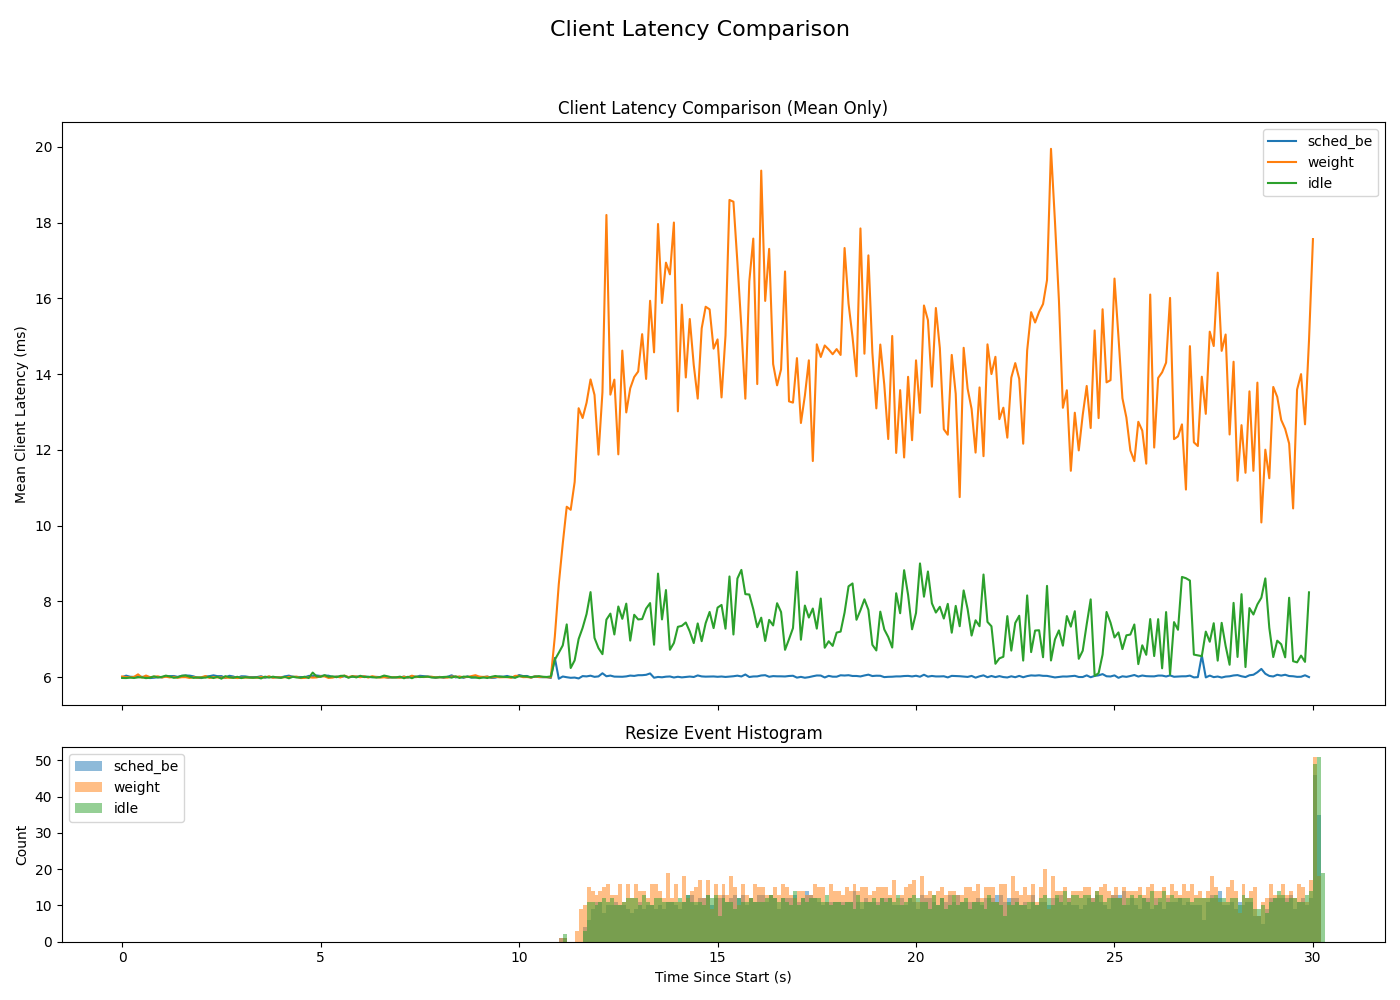
\includegraphics[width=\columnwidth]{graphs/srv-bg-cmp-all.png}
        \caption{Comparison of mean latency of the low load setting for weights,
        \schedidle{}, and \schedbe{}}\label{fig:srv-bg-cmp}
    \end{subfigure}
    \vspace{4pt}
    \caption{}\label{fig:srv-bg-idle}
\end{figure}

\begin{figure}[t]
    \centering
    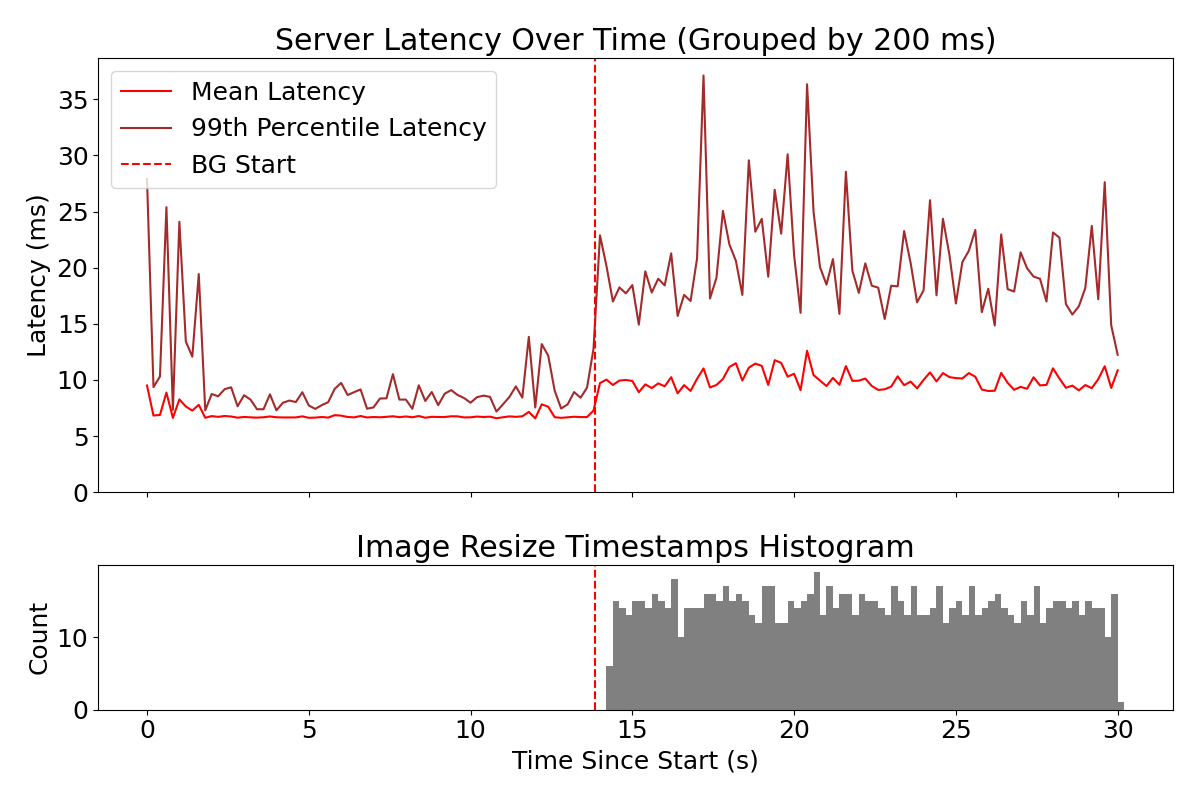
\includegraphics[width=\columnwidth]{graphs/kubernetes-idle.png}
    \caption{The same experiment as in \autoref{fig:kubernetes-unedited}, but
    running the BE as a \schedidle{} task}\label{fig:kubernetes-idle}
\end{figure}

\autoref{fig:srv-bg-idle} shows the result of running the BE jobs in the
microbenchmark in \schedidle{}, as well as a graph that compares the low load
setting of the standard \cgroups{} weight, \schedbe{}, and \schedidle{}. Average
latency still increases from $\sim$6ms to $\sim$8ms in the low load setting.
Although this increase is smaller than the original increase to $\sim$15ms using
the standard weight interface, it is still high compared to the 0ms increase
that \schedbe{} achieves. \autoref{fig:kubernetes-idle} shows similar results
for the Kubernetes experiment.
\section{Related work}

Some existing work focuses on isolating real-time applications in
Linux~\cite{rt-in-linux, state-rt-linux}, while Wasted Cores~\cite{wasted-cores}
focuses on the idle behavior of the Linux scheduler.

Other systems work around the kernel scheduler, by running primarily in
userspace~\cite{perfiso,caladan,skyloft}.

Linux's own \schedidle{} policy attempts to address this issue, but does not
fully solve it (running the microbenchmark using \schedidle{} still leads to an
increase in the mean latency from 6ms to 8).
%-------------------------------------------------------------------------------
\section{Conclusion}
%-------------------------------------------------------------------------------

This work shows that current isolation systems like Kubernetes are unable to
effectively performance isolate between LC and BE workloads for workloads that
are CPU-intensive. We trace this problem down to Linux's \cgroups{}, and show
that because Linux uses per-core runqueues, its weight-based interface for
isolation is not enforced across cores. Using a weight-based interface for
isolating LC and BE has other problems as well: it makes it hard to enforce a
split across cores, and it interacts poorly with the large scheduling quantum
that Linux uses.

Instead, we propose an API that separates BEs from LCs by introducing the
\beclass{} priority class. Enforcing \beclass{} requires less cross-core
interaction than a weight-based isolation approach, and ensures that no BE is
ever running when an LC is queued. During high load this requires `parking',
which enforces that BEs are immediately runnable once the load goes down, with
minimal interference for LCs in the meantime while the load is high.

We implement this strict priority in Linux, and show that the resulting
\schedbe{} allows \cgroups{} itself, as well as higher level applications that
build on \cgroups{} like Kubernetes, to do a better job of isolating LC from BE
workloads. Using \schedbe{} rather than the standard \cgroups{} weight interface
decrease the impact starting a BE process has on LC latencies from >2x to 0, and
under high load a parked \schedbe{} process running in a Kubernetes pod can
resume execution normally after multiple minutes of no user space CPU time.



%-------------------------------------------------------------------------------
%\bibliography{paper.bib}
\printbibliography

%%%%%%%%%%%%%%%%%%%%%%%%%%%%%%%%%%%%%%%%%%%%%%%%%%%%%%%%%%%%%%%%%%%%%%%%%%%%%%%%
\end{document}
%%%%%%%%%%%%%%%%%%%%%%%%%%%%%%%%%%%%%%%%%%%%%%%%%%%%%%%%%%%%%%%%%%%%%%%%%%%%%%%%

%%  LocalWords:  endnotes includegraphics fread ptr nobj noindent
%%  LocalWords:  pdflatex acks
